\documentclass[11pt]{amsart}
\usepackage{graphicx}
\graphicspath{{../figs/}}
\usepackage{amsmath}
\usepackage{amsthm}
\usepackage{amssymb}
\usepackage[letterpaper,top=2cm,bottom=2cm,left=2cm,right=2cm,marginparwidth=1.75cm]{geometry}
\usepackage{float}
\usepackage{hyperref}
\usepackage{cleveref}
\usepackage{algorithm}
\usepackage{algorithmic}

\newtheorem{definition}{Definition}

\usepackage{xcolor}
\newcommand{\mati}[1]{\textcolor{red}{#1}}
\newcommand{\CC}{\mathbb{C}}
\newcommand{\RR}{\mathbb{R}}
\newcommand{\PP}{\mathbb{P}}

\title{Obtaining the committor function in cryo-EM}
\author{Matias Andia}
\date{April 2026}

\begin{document}

\begin{abstract}
    Cryogenic electron microscopy (cryo-EM) provides a powerful window into the conformational heterogeneity of biological macromolecules, but extracting physically meaningful dynamical information from conformational distributions remains challenging. Recent methods, such as RECOVAR, compute an estimate of the conformational density in a low-dimensional principal component analysis (PCA) latent space, which, by Boltzmann statistics, encodes an effective free energy landscape. We propose using this landscape to compute the \emph{committor function} between pairs of conformational states identified by RECOVAR. The committor, satisfying a backward Kolmogorov equation, quantifies the probability that a macromolecule undergoing Langevin dynamics transitions to one state before another. Because the RECOVAR latent space is typically 4–10 dimensional, traditional numerical PDE solvers are intractable. We argue that the tensor train (TT) approach of \cite{committor} provides a natural remedy, enabling committor computation with complexity linear in the number of dimensions.
\end{abstract}

\maketitle

\section{Introduction}
Proteins and macromolecular complexes are not static objects but rather they populate a continuum of conformations, and the transitions between these conformations underlie virtually all biological functions. Cryo-EM, by imaging many individual particles in a vitrified state, offers snapshots of this conformational distribution. A central goal of cryo-EM heterogeneity analysis is therefore not merely to catalog conformational states, but to understand the dynamics between them.

In \cite{recovar}, Gilles and Singer present RECOVAR, which is a statistically rigorous approach to this problem of analyzing the heterogeneous distributions of conformations. It estimates a latent representation of the heterogeneous conformational distribution using a regularized covariance estimator and then reconstructs a conformational density in that latent space. This density gives access to stable states and the free energy landscape of the molecule via Boltzmann statistics. In this pipeline, this latent space gives us a reduced coordinate system in which the conformational landscape can be analyzed quantitatively, as we will soon see. 
 
Once this latent density is obtained, a natural next object is the \emph{committor function}. Put simply, the committor is the probability that a trajectory initialized at a given point reaches some state B before state A. For overdamped Langevin dynamics (which we assume the molecules in cryo-EM follow), the committor solves a backward Kolmogorov equation with Dirichlet boundary conditions on the two target sets. Naively, solving such a problem would have a computational and memory complexity that is exponential in dimension. In \cite{committor}, however, Chen et al. demonstrate that this problem can be written in a (soft) variational form, which can then be solved efficiently by representing the density and the committor in \emph{tensor train} (TT) form. From here, the committor can be obtained via a clever alternating least squares, resulting in both the computational and memory complexity scaling linearly with dimension.

Thus to apply such an algorithm in cryo-EM, one could imagine a general pipeline that would begin with using RECOVAR to infer a low-dimensional free-energy landscape in latent space. Then one would apply the tensor-train committor algorithm on that latent landscape to characterize the transition pathways between the conformational states. This would not only give us the stable states but also the transition-state structure of the molecule, as demonstrated in \Cref{subsec:cryo-res}.

\section{The RECOVAR Latent space and effective free energy}
\subsection{The RECOVAR pipeline}
RECOVAR starts from the cryo-EM image-formation model
\begin{align}
    y_i = P_i x_i + \epsilon_i, \qquad \epsilon_i \sim \mathcal{N}(0,\Lambda_i),
\end{align}
where $y_i$ is the observed 2D image, $x_i$ is the underlying 3D conformation, and $P_i$ combines projection, pose, and CTF effects. In this model, they take the poses $\phi_i$ to already be estimated (using, e.g., a consensus reconstruction) so that, using a regularized least-squares procedure, they estimate the covariance matrix $\hat{\Sigma}$ from
\begin{align}
    \hat{\Sigma}:=\operatorname*{arg\,min}_\Sigma\sum_{i=1}^n\|(y_i-P_i\hat{\mu})(y_i-P_i\hat{\mu})^*-(P_i\Sigma P_i^*+\Lambda_i)\|^2_F+\|\Sigma\|^2_R,
\end{align}
where $\|\cdot\|^2_F$ is the Frobenius norm, $\|A\|^2_R=\sum_{i,j}A^2_{i,j}R_{i,j}$ for $R$ the regularization weights, and $\hat{\mu}$ is the mean estimated from solving the linear least-squares problem
\begin{align}
    \hat{\mu}:=\operatorname*{arg\,min}_\mu\sum_{i=1}^n\|y_i-P_i\mu\|^2_{\Lambda_i^{-1}}+\|\mu\|^2_w\quad\text{where } \|v\|^2_w=\sum_i|v_i|^2w_i\quad \&\quad\|v\|^2_{\Lambda_i^{-1}}=v^*\Lambda_i^{-1}v.
\end{align}
The $d$-leading eigenvectors of $\hat{\Sigma}\in\CC^{N^3\times N^3}$ are then used to form $U\in\CC^{N^3\times d}$, defining the principal components. Hence we can embed each conformation $x_i$ into latent coordinates as
\begin{align}
    z_i=U^*(x_i-\hat{\mu})\in\RR^d.
\end{align}
Further, because $U$ is orthogonal, distance between conformations in volume space are preserved up to truncation error, i.e. $\|x_i-x_j\|^2\approx\|z_i-z_j\|^2$.

\subsection{Conformational density and free energy}\label{subsec:rec-con-dens}
These RECOVAR latent coordinates provide a low-dimensional space in which the conformational distribution of the dataset can be estimated directly. In practice, this is done by applying kernel density estimation (see \Cref{sec:fut} for further discussion on this) to the embedded samples $\{z_i\}_{i=1}^n$, yielding an empirical density $\hat{\rho}(z)$. This density is not itself a physical Boltzmann density in the strict sense, but it provides an effective description of how frequently different regions of latent space are occupied by the conformational ensemble represented in the dataset.

It is therefore natural to define an associated effective free energy landscape by
\begin{align}
    F(z) := -\beta^{-1}\log \hat{\rho}(z) + C,
\end{align}
where $\beta=1/T$ and $C$ is an arbitrary additive constant. Regions of high conformational density correspond to low values of $F$, while low-density regions correspond to energetic barriers separating distinct basins. In this sense, metastable conformational states appear as local minima of the effective free energy, and transitions between them occur through the intervening high-free-energy regions.

Once the conformational distribution has been reduced to a tractable latent density, one may pose the committor problem on this latent space, making this interpretation is particularly useful for our purposes. The resulting committor then quantifies the probability that a trajectory initiated at a given latent configuration first reaches one metastable basin rather than another, thereby giving a notion of how a molecule may progress through its conformational states.

\section{Obtaining the committor function}
\subsection{What we need to solve}
Recall that we are interested in the overdamped Langevin process
\begin{align}
    d\boldsymbol{X}_t=-\nabla V(\boldsymbol{X}_t)dt+\sqrt{2\beta^{-1}}d\boldsymbol{W}_t,
\end{align}
where $\boldsymbol{X}_t\in\Omega\subset\RR^d$ is the state of the system, $V:\Omega\to\RR$ is a smooth, potential energy function, $\beta=1/T$ is the inverse of the temperature, and $\boldsymbol{W}_t$ is a $d$-dimensional Wiener process. For a potential function $V$ that is confining on $\Omega$, letting $Z_\beta=\int_\Omega\exp(-\beta V(\boldsymbol{x}))d\boldsymbol{x}$ be the partition function, one then sees that the equilibrium probability distribution of these dynamics is the Boltzmann-Gibbs distribution
\begin{align}
    p(\boldsymbol{x})=\frac{1}{Z_\beta}\exp(-\beta V(\boldsymbol{x})).
\end{align}
As in the case of conformational heterogeneity in cryo-EM, we are interested in the transition between two simply connected domains $A,B\subset\Omega$ that have smooth boundaries and are disjoint. To investigate this, we define the committor function $q:\Omega\to[0,1]$ as
\begin{align}
    q(\boldsymbol{x})=\PP(\tau_A<\tau_B:\boldsymbol{X}_0=\boldsymbol{x}),
\end{align}
where $\tau_A$ and $\tau_B$ are the times it takes for our process to first hit $A$ and $B$, respectively. Computing this function comes from solving the following backward Kolmogorov equation with Dirichlet boundary conditions
\begin{align}
    -\beta^{-1}\Delta q(\boldsymbol{x})+\nabla V(\boldsymbol{x})\cdot\nabla q(\boldsymbol{x})=0 \ \text{in}\ \Omega\backslash(A\cup B), \ q(\boldsymbol{x})|_{\partial A}=0,\ q(\boldsymbol{x})|_{\partial B}=1.
\end{align}
A careful analysis (see, e.g., \cite{varCommitt}) then shows that this can be rewritten as a variational problem, enforcing the boundary conditions as penalty terms
\begin{align}
    \operatorname*{arg\,min}_q\int_\Omega|\nabla q(\boldsymbol{x})|^2p(\boldsymbol{x})d\boldsymbol{x}+\rho\int_{\partial A}q(\boldsymbol{x})^2p_{\partial A}(\boldsymbol{x})d\boldsymbol{x}+\rho\int_{\partial B}(q(\boldsymbol{x})-1)^2p_{\partial B}(\boldsymbol{x})d\boldsymbol{x},
\end{align}
where $p_{\partial A}$ and $p_{\partial B}$ are just $p$ supported on $\partial A$ and $\partial B$ respectively. These boundary measures break the TT structure, however, because they are not absolutely continuous with respect to the Lesbesgue measure. This means that this formulation is not directly compatible with optimization even when one assumes $q$ to have TT form. So, as in \cite{committor}, we consider the \emph{soft committor function}
\begin{align}\label{eq:tt-cmmttr}
    \operatorname*{arg\,min}_q\int_\Omega|\nabla q(\boldsymbol{x})|^2p(\boldsymbol{x})d\boldsymbol{x}+\rho\int_\Omega q(\boldsymbol{x})^2p_A(\boldsymbol{x})d\boldsymbol{x}+\rho\int_\Omega (q(\boldsymbol{x})-1)^2p_B(\boldsymbol{x})d\boldsymbol{x},
\end{align}
where $p_A$ and $p_B$ are probability densities that are absolutely continuous with respect to the Lebesgue measure on $\Omega$. In what follows we will refer to soft committor functions as committor functions, as they admit similar probabilistic interpretations. For a more thorough analysis of this we refer the reader to Appendix A of \cite{committor}.

\subsection{Reformulating this}
A key ingredient to solving this efficiently is the \emph{tensor train} (TT) approximation defined as follows.
\begin{definition}
    Let $\mathcal{A}\in\RR^{n_1\times\cdots\times n_d}$ be a $d$-way tensor with entries indexed by $(i_1,\ldots,i_d)$. We say that $\mathcal{A}$ is a TT with ranks $\boldsymbol{r}=(r_0,\ldots,r_d)$ where $r_0=r_d=1$ if one can write
    \begin{align}
        \mathcal{A}(i_1,\ldots,i_d)=\sum_{\alpha_0,\ldots,\alpha_d=1}^{r_0,\ldots,r_d}\mathcal{G}_1(\alpha_0,i_1,\alpha_1)\cdots\mathcal{G}_d(\alpha_{d-1},i_d,\alpha_d)=\mathcal{G}_1(:,i_1,:)\cdots\mathcal{G}_d(:,i_d,:)
    \end{align}
    for all $(i_1,\ldots,i_d)$, where we note $\mathcal{G}_k(:,i_k,:)\in\RR^{r_{k-1}\times r_k}$. The 3-way tensor $\mathcal{G}_k\in\RR^{r_{k-1}\times n_k\times r_k}$ is called the $k$-th core of $\mathcal{A}$.
\end{definition}

Following Section 3 of \cite{committor}, we now obtain the committor function by solving \cref{eq:tt-cmmttr}, assuming that $q$ has a TT parametrization. We show that by approximating the equilibrium probability distribution $p$ in this format, the optimization problem can be solved using a standard alternating least squares approach.

Writing our domain like $\Omega=\Omega_1\times\cdots\Omega_d$, we let $\{\phi^{(k)}_j\}^\infty_{j=1}$ be an orthogonal basis for each $L^2(\Omega_k)$. To make this problem finite dimensional, we consider the subspace of $L^2(\Omega_k)$ spanned by the first $L^{(k)}$ basis functions. We then consider an expansion of $q$ in this tensor product basis
\begin{align}
    q(\boldsymbol{x})=\sum_{\boldsymbol{i}}\mathcal{Q}(\boldsymbol{i})\phi_{i_1}^{(1)}(x_1)\cdots\phi_{i_d}^{(d)}(x_d),
\end{align}
where we defined $\boldsymbol{i}=(i_1,\ldots,i_d)$. Using this, we can rewrite the optimization problem as
\begin{align}\label{eq:full-tt-cmmttr}
    \operatorname*{arg\,min}_\mathcal{Q}\sum_{k=1}^d\sum_{\boldsymbol{i},\boldsymbol{j}}H^k(\boldsymbol{i};\boldsymbol{j})\mathcal{Q}(\boldsymbol{i})\mathcal{Q}(\boldsymbol{j})+\rho\sum_{\boldsymbol{i},\boldsymbol{j}}H^A(\boldsymbol{i};\boldsymbol{j})\mathcal{Q}(\boldsymbol{i})\mathcal{Q}(\boldsymbol{j})+\rho\sum_{\boldsymbol{i},\boldsymbol{j}}H^B(\boldsymbol{i};\boldsymbol{j})\mathcal{Q}(\boldsymbol{i})\mathcal{Q}(\boldsymbol{j})-2\rho\sum_{\boldsymbol{i}}\mathcal{Q}(\boldsymbol{i})h^B(\boldsymbol{i})+\rho,
\end{align}
where the first and second terms equal the first and second terms of \cref{eq:tt-cmmttr} respectively, the last three terms equal the third term of \cref{eq:tt-cmmttr}, and we defined
\begin{align}
    &H^k(\boldsymbol{i};\boldsymbol{j})=\int_\Omega\frac{\partial}{\partial x_k}\left[\phi_{i_1}^{(1)}(x_1)\cdots\phi_{i_d}^{(d)}(x_d)\right]\frac{\partial}{\partial x_k}\left[\phi_{j_1}^{(1)}(x_1)\cdots\phi_{j_d}^{(d)}(x_d)\right]p(\boldsymbol{x})d\boldsymbol{x}\\
    &H^{A,B}(\boldsymbol{i};\boldsymbol{j})=\int_\Omega\phi_{i_1}^{(1)}(x_1)\cdots\phi_{i_d}^{(d)}(x_d)\phi_{j_1}^{(1)}(x_1)\cdots\phi_{j_d}^{(d)}(x_d)p_{A,B}(\boldsymbol{x})d\boldsymbol{x}\\ 
    &h^{B}(\boldsymbol{i})=\int_\Omega\phi_{i_1}^{(1)}(x_1)\cdots\phi_{i_d}^{(d)}(x_d)p_B(\boldsymbol{x})d\boldsymbol{x}.
\end{align}
Computing these tensors explicitly is of course intractible, as it requires integration over $\Omega\subset\RR^d$ and storing tensors of size exponential in $d$. We now show how we can use TT approximations to obtain these tensors and solve \cref{eq:full-tt-cmmttr} with computational and storage complexities that scale linearly in $d$.

\subsection{Constructing the tensors efficiently} Let's begin by constructing $H^k$, assuming that the equilibrium density can be approximated in TT form, i.e.
\begin{align}\label{eq:tt-basis}
    p(\boldsymbol{x})=\sum_{\substack{m_1,\ldots,m_d\\ \alpha_0,\ldots,\alpha_d}}\mathcal{P}_1(\alpha_0,m_1,\alpha_1)\cdots\mathcal{P}_d(\alpha_{d-1},m_d,\alpha_d)\psi^{(1)}_{m_1}(x_1)\cdots\psi^{(d)}_{m_d}(x_d),
\end{align}
where $\{\psi^{(k)}_j\}^{K^{(k)}}_{j=1}$ are univariate basis functions $\Omega_k\to\RR$ and $\mathcal{P}_k\in\RR^{r_{k-1}\times K^{(k)}\times r_k}$ is the coefficient tensor core for $k=1,\ldots,d$ (in general, if we say that a function has a TT form, we simply mean that it can be expressed in this way). Hence we can split up our $d$-dimensional integral into a sum and product of 1-dimensional integrals. More precisely, for $\ell=1,\ldots,d$, defining
\begin{align}
    A_\ell(\alpha_{\ell-1},\alpha_\ell):=\int_{\Omega_\ell}f_\ell(x_\ell)\mathcal{P}_\ell(\alpha_{\ell-1},m_\ell,\alpha_\ell)\psi^{(\ell)}_{m_\ell}(x_\ell)dx_\ell\quad\text{where }f_\ell(x_\ell)
    =\begin{cases}\phi^{(\ell)}_{i_\ell}(x_\ell)\,\phi^{(\ell)}_{j_\ell}(x_\ell), & \ell \neq k,\\
    \frac{\partial\phi^{(\ell)}_{i_\ell}}{\partial x_\ell}\frac{\partial\phi^{(\ell)}_{j_\ell}}{\partial x_\ell}, & \ell = k,
    \end{cases}
\end{align}
we can write $H^k=A_1\cdots A_d$. Because the shape of these $d$ matrices is independent of dimension, we see that this computation of $H^k$ scales linearly in $d$. Many of these $A_\ell$ can clearly be reused for other $k$ so it is not difficult to see that we can compute $\{H^k\}^d_{k=1}$ in time that scales linearly with the dimension. Letting $K:=\max_\ell K^{(\ell)},\ L:=\max_\ell L^{(\ell)},$ and $r=\max_\ell r_\ell$, a careful analysis shows that in this form, $\{H^k\}^d_{k=1}$ can be computed with a computational cost of $\mathcal{O}(dr^2KL^2)$ and a memory complexity of $\mathcal{O}(dKL^2+dr^2L^2)$ (including the storage of intermediary tensors).

The construction for $H^A$ and $H^B$ is essentially the same except now we are representing $p_A$ and $p_B$ in TT format. This representation is justified because in high dimensions the equilibrium density concentrates so that most of the probability mass lies on a thin shell and correlations between these shells are weak (for spheres this is captured by the Gaussian annulus theorem). As a result $p_A$ and $p_B$ retain  low-rank TT approximations. For a more careful consideration of this, we refer the reader to Section 3.3 of \cite{committor}. From here we basically just apply the analysis done for $H^k$ and letting $s$ be the maximal rank of the cores used to represent $p_A$ and $K_A$ be the maximal number of basis modes, we obtain a time complexity of $\mathcal{O}(ds^2K_AL^2)$ to compute $H^A$. Defining similar things for $B$, we obtain a time complexity of $\mathcal{O}(dt^2K_BL^2)$ for computing $H^B$. The memory complexities are $\mathcal{O}(dK_AL^2+ds^2L^2)$ and $\mathcal{O}(dK_BL^2+dt^2L^2)$ respectively.

Lastly, using this TT approximation for $p_B$, we can obtain $h^B$ in a similar way with computational and memory complexities of $\mathcal{O}(dt^2K_BL)$ and $\mathcal{O}(dK_BL+dt^2L)$ respectively. Now that all of these tensors are in TT form, we may turn to actually solving the minimization problem \cref{eq:full-tt-cmmttr}.

\subsection{Optimization}
Before tackling this, we still must approximate the coefficient tensor in TT format as
\begin{align}
    \mathcal{Q}(\boldsymbol{i}):=\sum_{\alpha_0,\ldots,\alpha_d}\mathcal{Q}_1(\alpha_0,i_1,\alpha_1)\cdots\mathcal{Q}_d(\alpha_{d-1},i_d,\alpha_d).
\end{align}
We can now solve the minimization from \cref{eq:full-tt-cmmttr} by an alternating least squares (ALS) approach. That is, in each ALS iteration, we loop over the dimensions $k=1,\ldots,d$. At step $k$, we treat all coefficient cores but $\mathcal{Q}_k$ as constant, giving us an unconstrained least squares problem for $\mathcal{Q}_k$. Naively, the computational complexity would be $\mathcal{O}(d^2)$ since we must sum $d$ terms, each of which requires $\mathcal{O}(d)$ tensor contractions. Using the same trick as in the computation of $H^k$, the computational complexity can be brought down to $\mathcal{O}(d)$.

Hence, we obtain the key result of this algorithm: \emph{using TT factorizations, the committor function can be computed by solving \cref{eq:full-tt-cmmttr} with a computational and memory complexity that scales linearly in the dimension}.

\subsection{Connecting this to RECOVAR}
The RECOVAR latent space is a very natural setting for this method. The embedding dimension is small enough that the committor problem is meaningful, but still large enough that direct PDE discretization is far too expensive. A tensor-train method therefore sits in exactly the right regime because it is flexible enough to represent nontrivial transition geometry, but structured enough to avoid the curse of dimensionality. In practice, an example pipeline could be as follows.
\begin{enumerate}
    \item Use RECOVAR to estimate the latent coordinates and density (maybe already in TT format, see \Cref{sec:fut}).
    \item Define metastable sets $A$ and $B$ in that latent space.
    \item Construct a TT approximation of the density (maybe not needed) and the soft boundary measures.
    \item Solve the variational committor problem by ALS.
    \item Extract transition pathways and transition-state regions from the resulting committor.
\end{enumerate}

\section{Results}
The code for these results can be found in the \texttt{quickstart.ipynb} notebook at \url{https://github.com/matias-ma/committor-tt}. We note that the implementation in this repository is a proof-of-concept and lacks full robustness. We also note that in the applications below, we found that many of the results are very sensitive to parameter selection. With a more careful parameter selection, some of the results below can likely be improved upon.

\subsection{Double-well}
As a sanity check for our implementation of the above algorithm, we consider a separable $d$-dimensional double-well model in which each coordinate experiences the same quartic potential
\begin{equation}
    V(x) = (x^2-1)^2,
\end{equation}
so that the full equilibrium density factorizes exactly as
\begin{equation}
    p(\boldsymbol{x}) \propto \prod_{\ell=1}^d \exp\!\bigl(-\beta V(x_\ell)\bigr)
    = \exp\!\Bigl(-\beta \sum_{\ell=1}^d (x_\ell^2-1)^2\Bigr).
\end{equation}
This is a particularly convenient test problem because the density has exact product structure, so the tensors appearing in the variational formulation admit low-rank TT approximations, yet the resulting committor still has a nontrivial transition layer between the two metastable basins.

We define the two metastable states to be sets that are small neighborhoods around the two wells,
\begin{equation}
    \boldsymbol{x}_A = (-1,\dots,-1), \qquad \boldsymbol{x}_B = (+1,\dots,+1),
\end{equation}
and replace the sharp indicators of $A$ and $B$ by smooth Gaussian product weights centered at these points (i.e. $p_A$ and $p_B$ are taken to be separable Gaussian densities that concentrate around $\boldsymbol{x}_A$ and $\boldsymbol{x}_B$, respectively). In the code, the width parameter $\sigma$ controls the size of these soft metastable neighborhoods. The parameter $\rho$ plays the role of a penalty weight in the variational formulation, enforcing the boundary conditions associated with the committor more strongly as $\rho$ increases.

We then solve the committor problem in two ways. First, we compute the full $d=4$ TT approximation using a Legendre basis on the box $[-2,2]^4$. Second, we solve the corresponding one-dimensional double-well problem on $[-2,2]$ using a higher-resolution Legendre approximation, which serves as a reference solution. To compare the two, we evaluate the 4-dimensional committor along the diagonal slice $(x,x,x,x), \ x \in [-1,1]$,
and plot this against the one-dimensional reference committor.

This benchmark is useful for several reasons. First, it verifies that the TT solver reproduces the expected transition profile in a setting where the underlying density is completely separable. Second, because the 4D problem is already beyond the range of naive grid-based discretization, it demonstrates that the TT approach can solve a genuinely higher-dimensional committor problem at modest cost. 

We note that these results are slightly different from those reported in \cite{committor} because we use different bases. In their example, they use a specialized basis tailored to the double-well experiment, while we use a simple Legendre basis. Nevertheless, the qualitative profile and the location of the transition region match their results rather well.

\begin{figure}[H]
    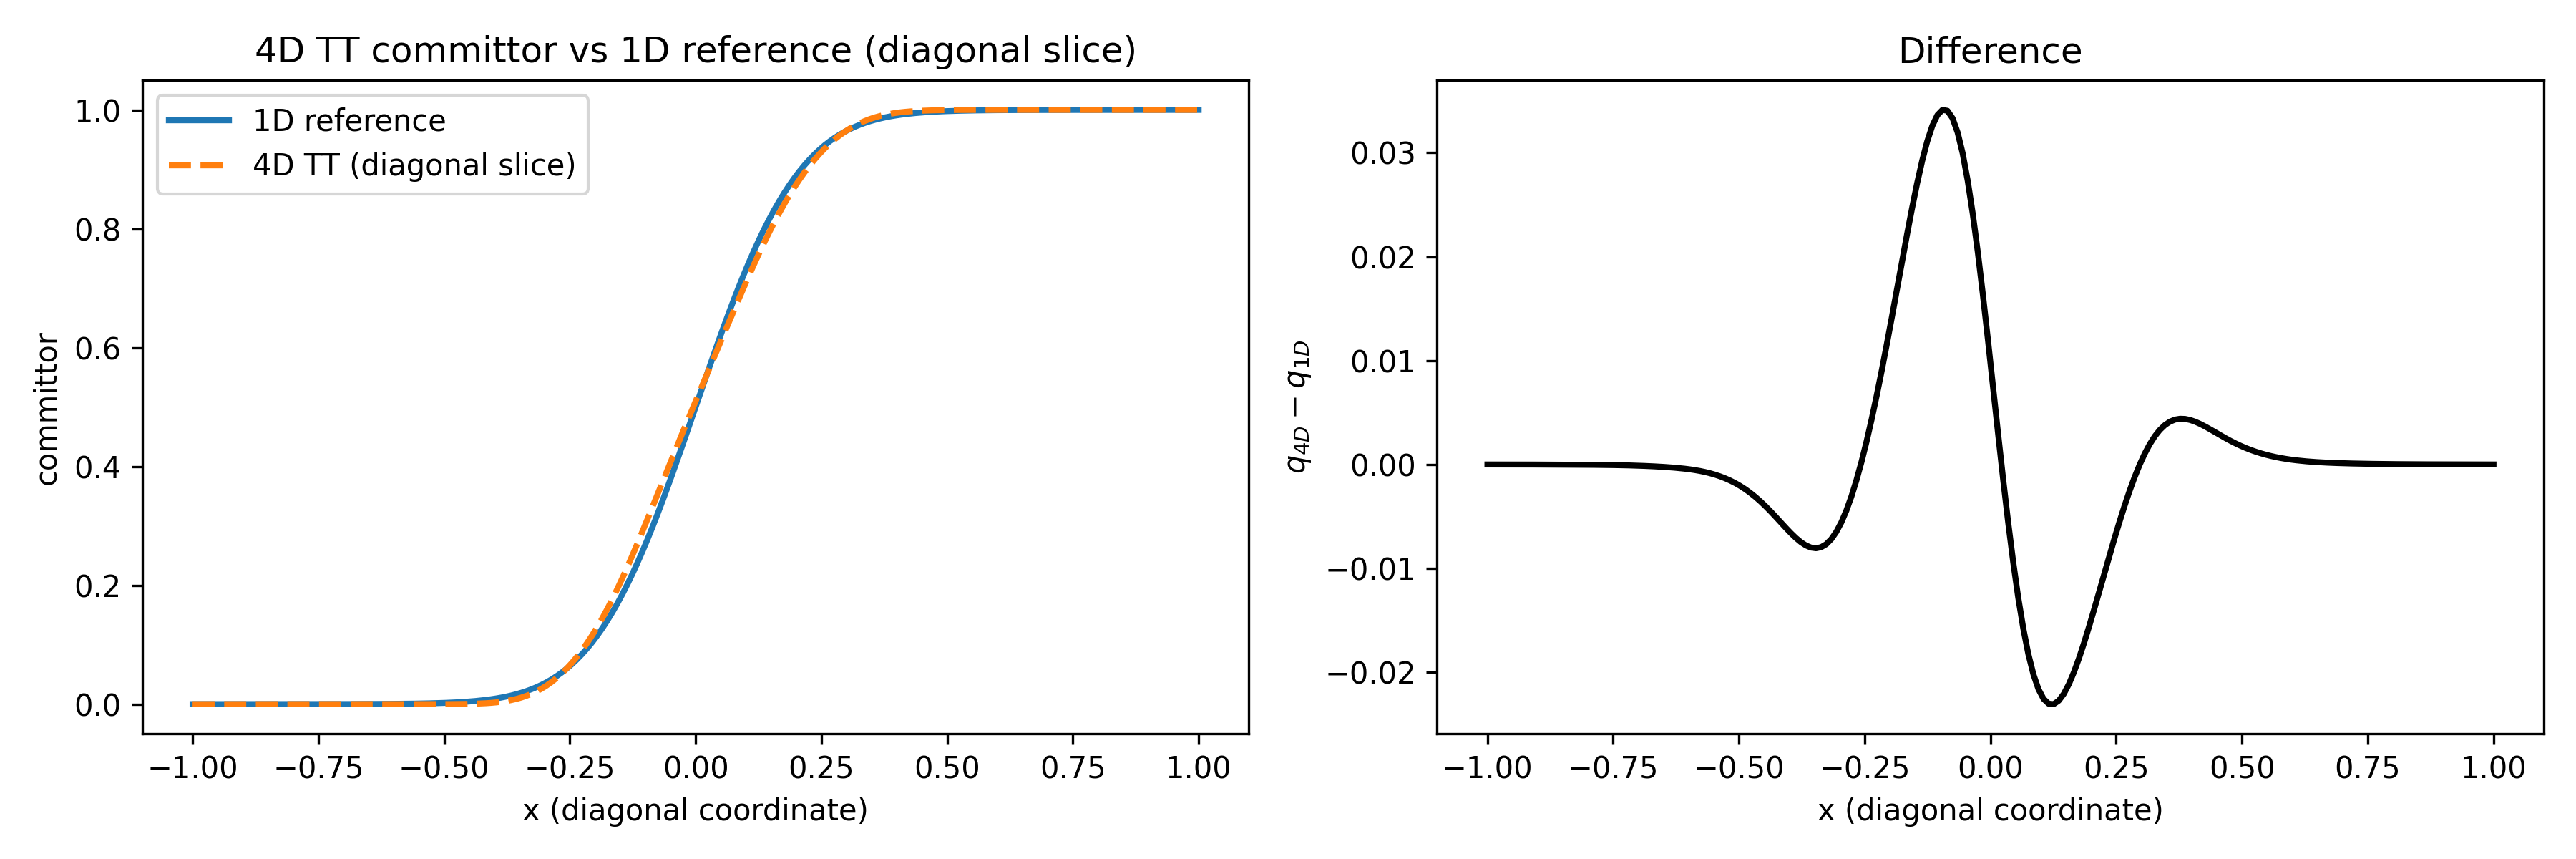
\includegraphics[scale=0.38]{dw_test.png}
    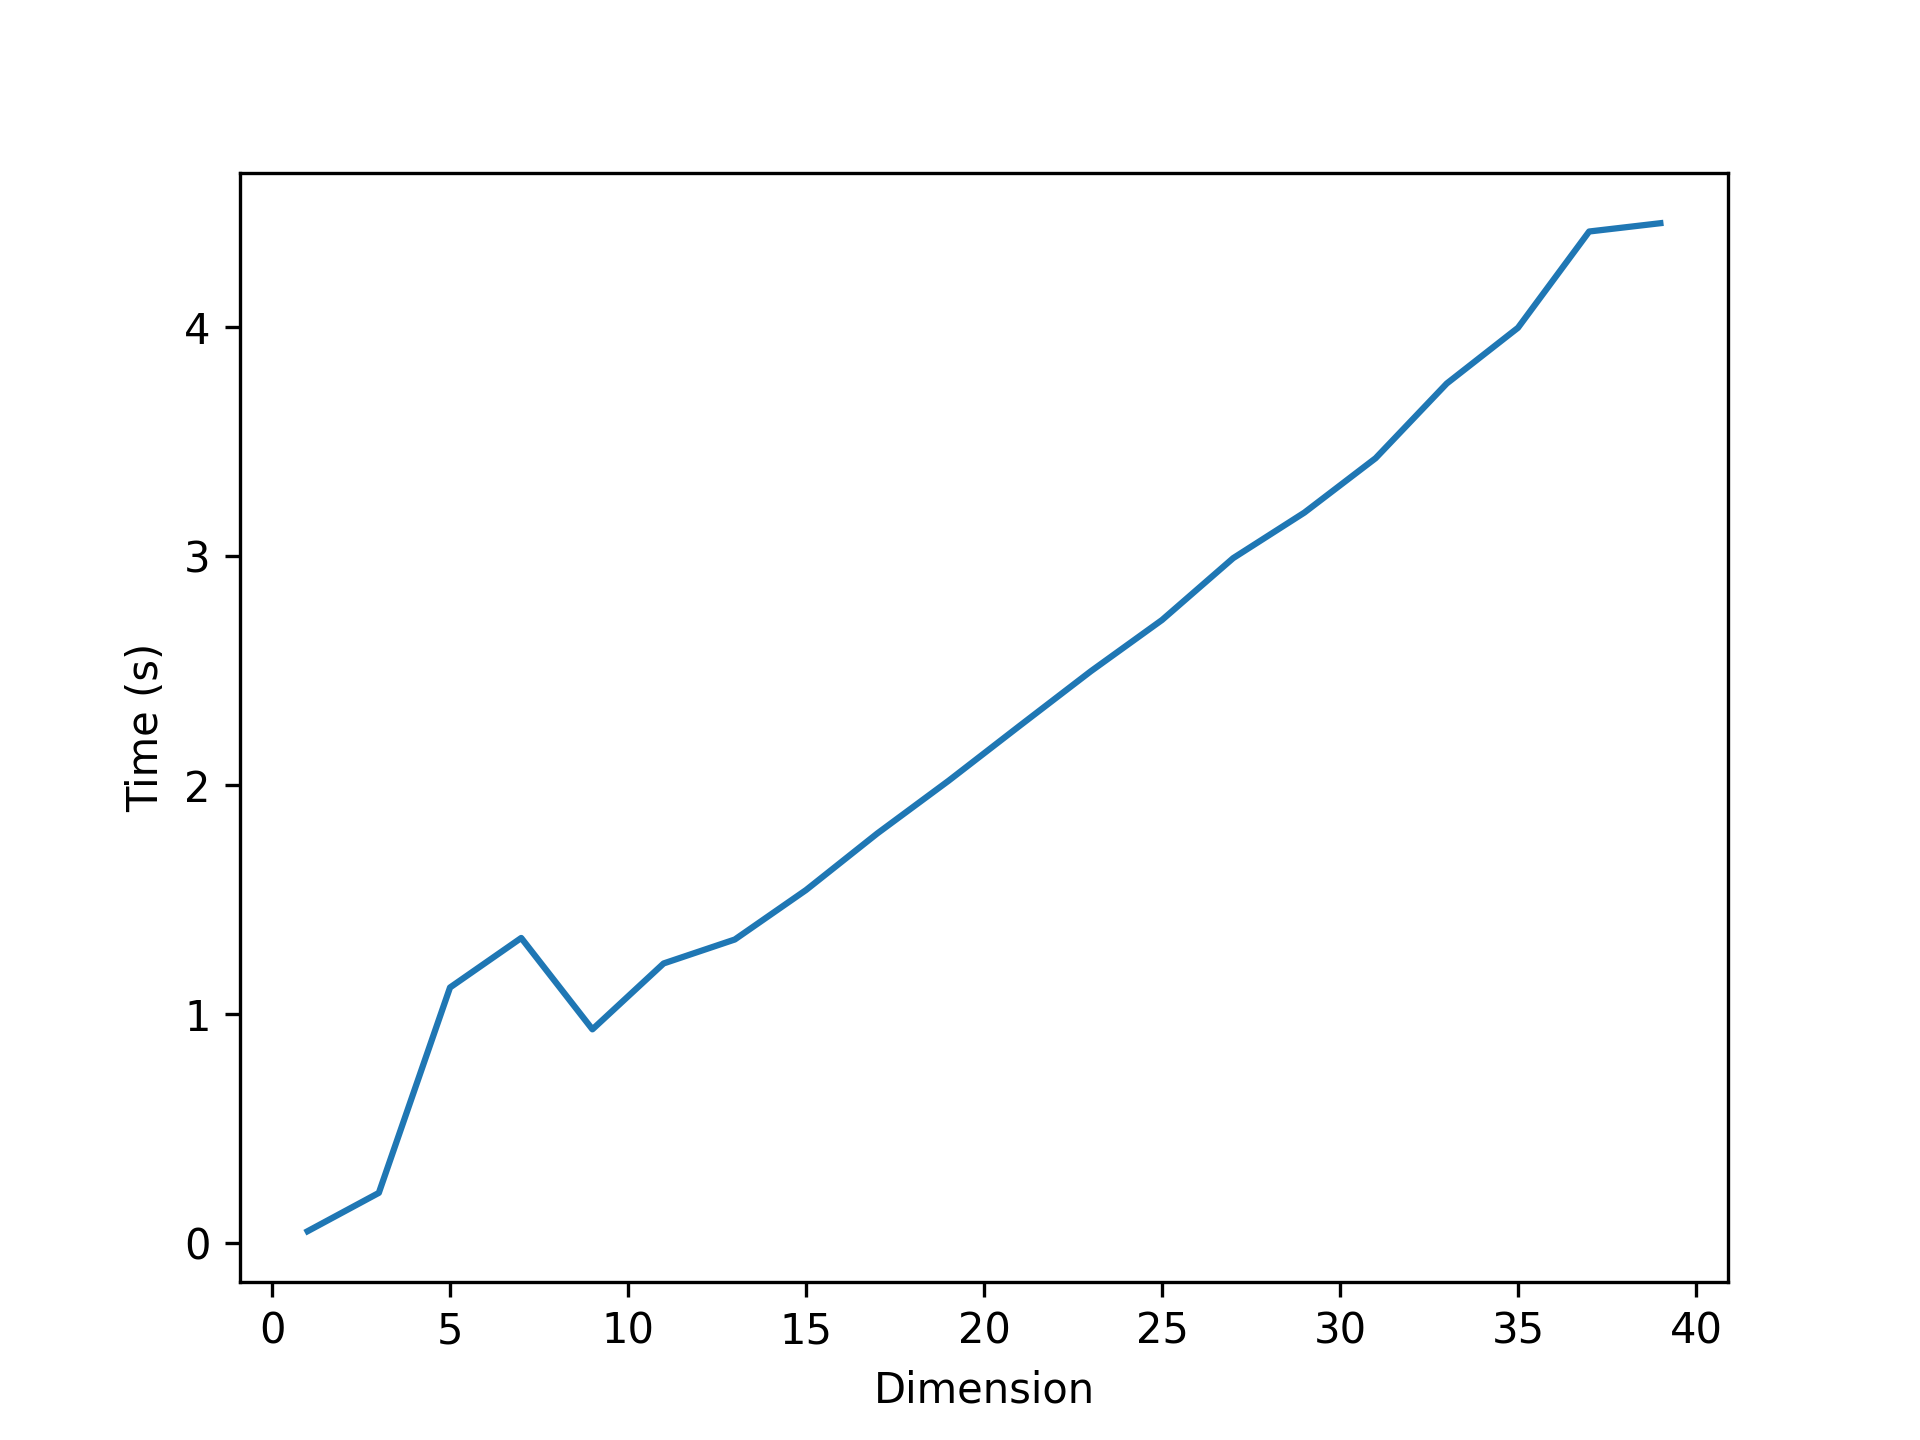
\includegraphics[scale=0.35]{dw_timing.png}
    \caption{This example demonstrates that for a toy example this algorithm works as expected. We note that any differences between these results and the ones from Section 4.1 of \cite{committor} arise from the fact that they use a special basis and we just used a simple Legendre basis.}
\end{figure}

\subsection{Toy RECOVAR example}\label{subsec:cryo-res}
Finding an interesting example for this was nontrivial without a tensor train approximation algorithm (i.e. you have to build the function from the ground up in tensor train form). Our primary goal was to come up with a conformational density and metastable states that look like they could come from a RECOVAR latent space embedding (see, e.g., Figure 3 of \cite{recovar}). In this we had some success but there is still lots of room for improvement.

To construct a conformational density that minimally captures the essential features, we worked in a two-dimensional latent space $z=(z_1,z_2)\in[-1.5,1.5]^2$ and define an equilibrium density as a uniform mixture of $N$ Gaussian components with centers $\{(c_j^1,c_j^2)\}^N_{j=1}$ are sampled along the curve $(c_j^1,c_j^2)=(\sin t_j, \sin 2t_j)$ for $t_j=2\pi j/N$. Because each component is separable, we can write this distribution as
\begin{align}\label{eq:toy-dens}
    \hat{\rho}(z)=\frac{1}{N}\sum_{i=1}^N\exp\left(-\frac{(z_1-c_i^1)^2}{\sigma^2}\right)\exp\left(-\frac{(z_2-c_i^2)^2}{\sigma^2}\right),
\end{align}
meaning that $\hat{\rho}$ has a rank-$N$ TT representation of the form \cref{eq:tt-basis} (critically, this differs from the double-well example because it is not exactly separable). The two metastable states are then taken to be Gaussians centered at $A=(-1,0)$ and $B=(1,0)$, which serve as the two end states of the figure-8 transition pathway. Equivalently, one may view these as the low-free-energy regions selected to define the committor boundary conditions, with effective free energy $F(z)=-\beta^{-1}\log \hat{\rho}(z)$.

\begin{figure}[H]
    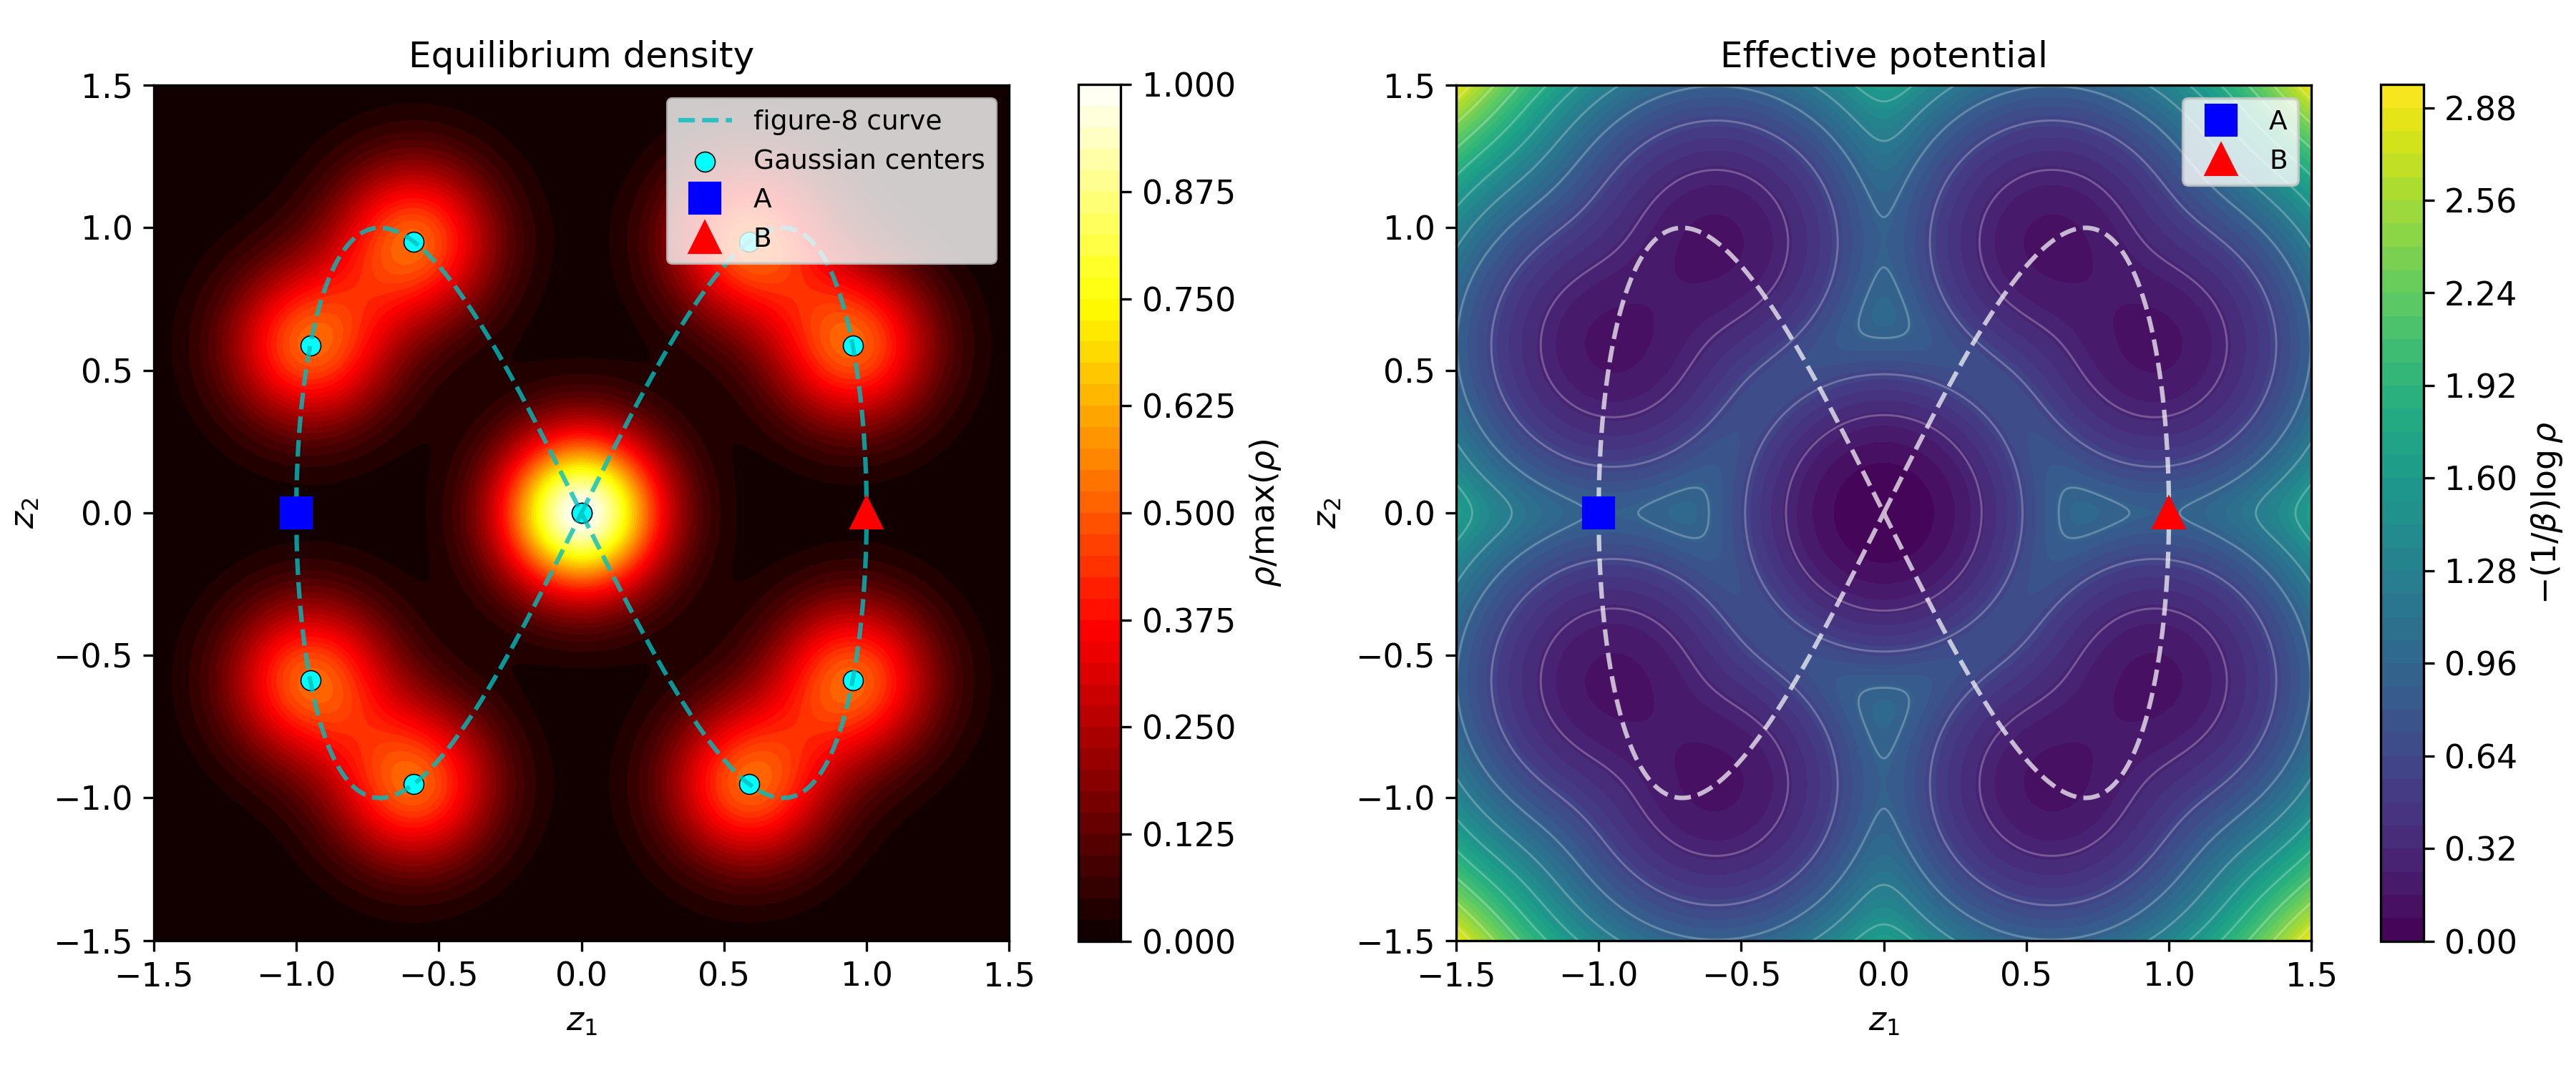
\includegraphics[scale=0.35]{toy_recovar_setup.png}
    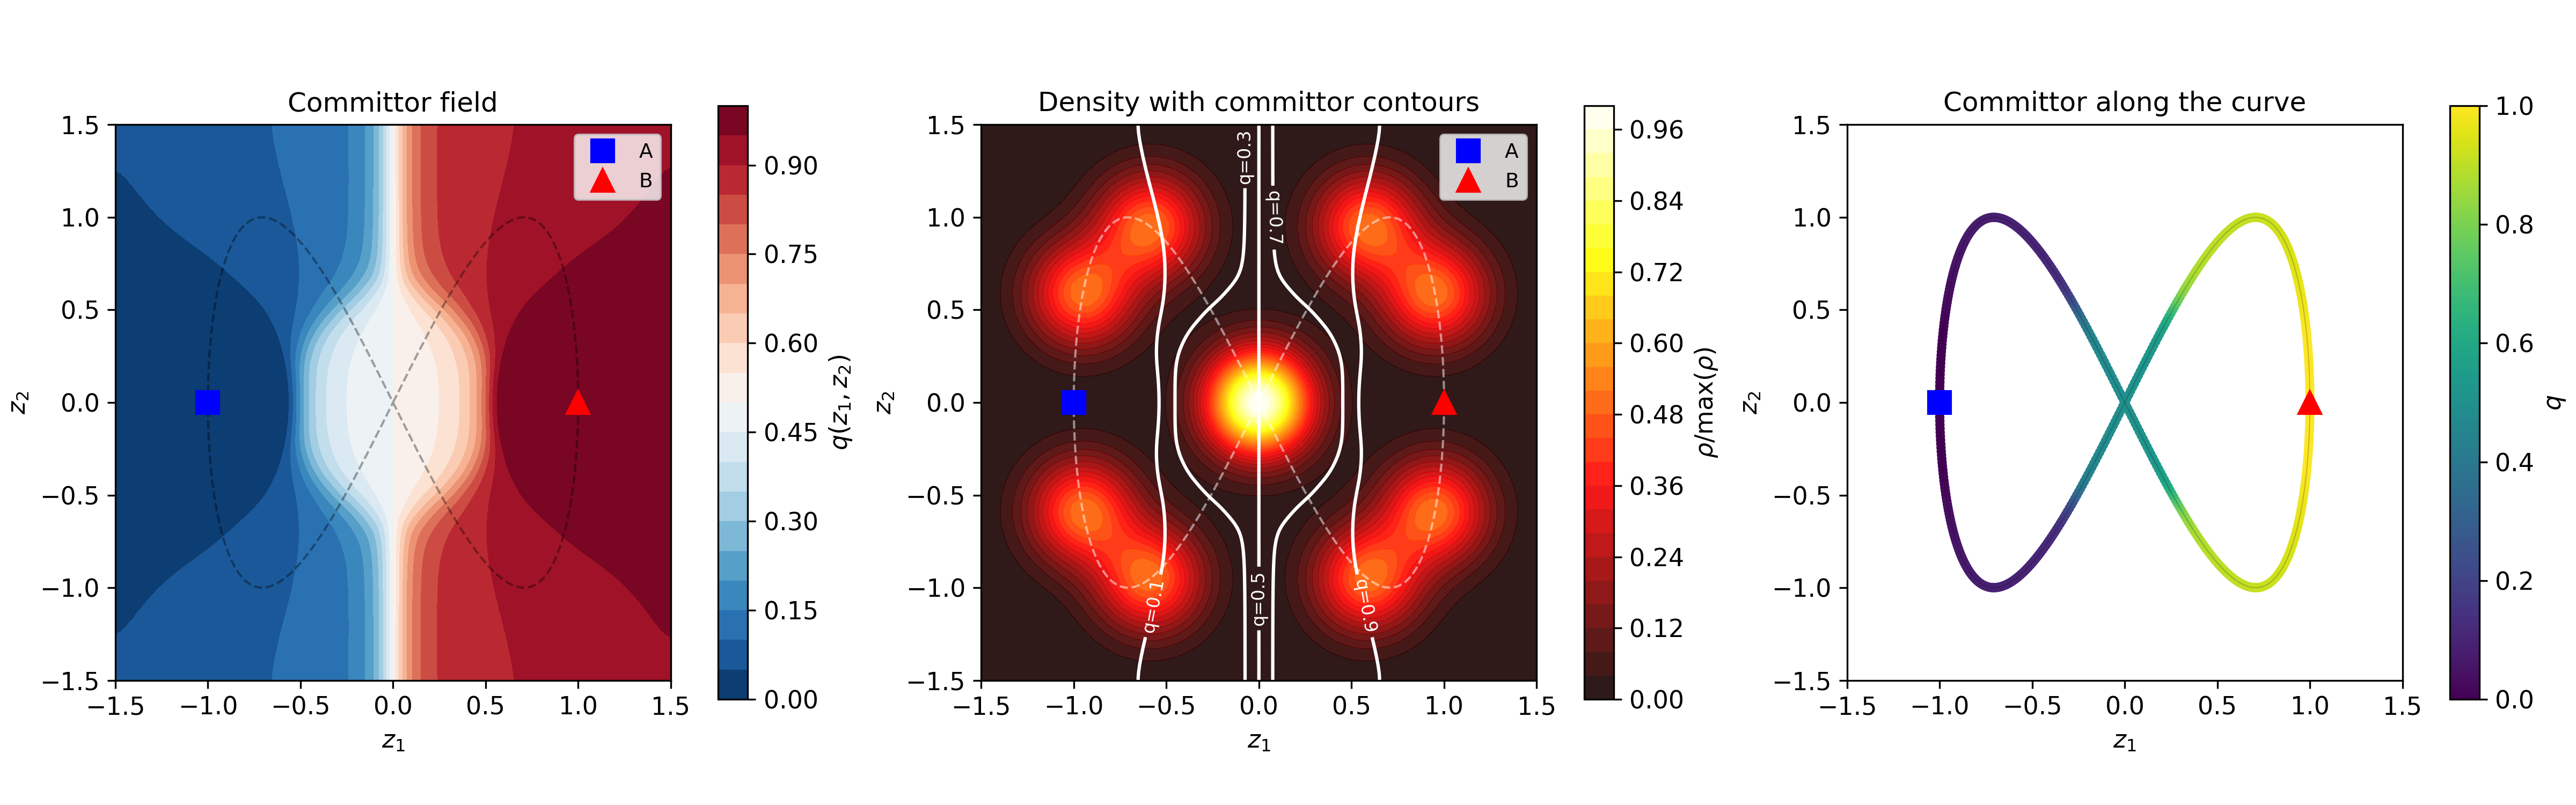
\includegraphics[scale=0.4]{recovar_2d.png}
    \caption{The 2 dimensional toy example with $N=10$. In the top panel we simply plot \cref{eq:toy-dens}. In the bottom panel we plot the committor function values obtained using the TT algorithm. Qualitatively, these plots agree with what one would generally expect.}
\end{figure}

While the two-dimensional version of this toy problem is primarily useful as a sanity check, the more interesting case is the higher-dimensional extension. In two dimensions, this problem can still be solved by classical numerical approaches, so the TT-based formulation is not yet being pushed to its limits. The four-dimensional setting is already much more representative of the high-dimensional regimes that motivate RECOVAR-like latent spaces, and it is here that tensor-train methods become genuinely useful. In this case we consider the density
\begin{align}
    \hat{\rho}(z)=\frac{1}{N}\sum_{i=1}^N\exp\left(-\frac{(z_1-c_i^1)^2}{\sigma^2}\right)\exp\left(-\frac{(z_2-c_i^2)^2}{\sigma^2}\right)\exp\left(-\frac{(z_3-c_i^3)^2}{\sigma^2}\right)\exp\left(-\frac{(z_4-c_i^4)^2}{\sigma^2}\right).
\end{align}
We were able to implement this extension and obtain qualitatively reasonable results, which suggests that the example does capture some of the intended geometry of a low-dimensional conformational manifold embedded in a higher-dimensional state space.

That said, this implementation should be interpreted cautiously. In its present form, it does not scale as cleanly as one would hope. The computation was expensive and, in several runs, took significantly longer than expected to converge. This appears to reflect the fact that the example is somewhat delicate to construct directly in tensor-train form, especially without a dedicated TT approximation procedure. Nevertheless, the resulting density and committor profiles look broadly consistent with the intended figure-8 transition picture, so we include them here as a proof-of-concept rather than as a fully optimized benchmark.
\begin{figure}[H]
    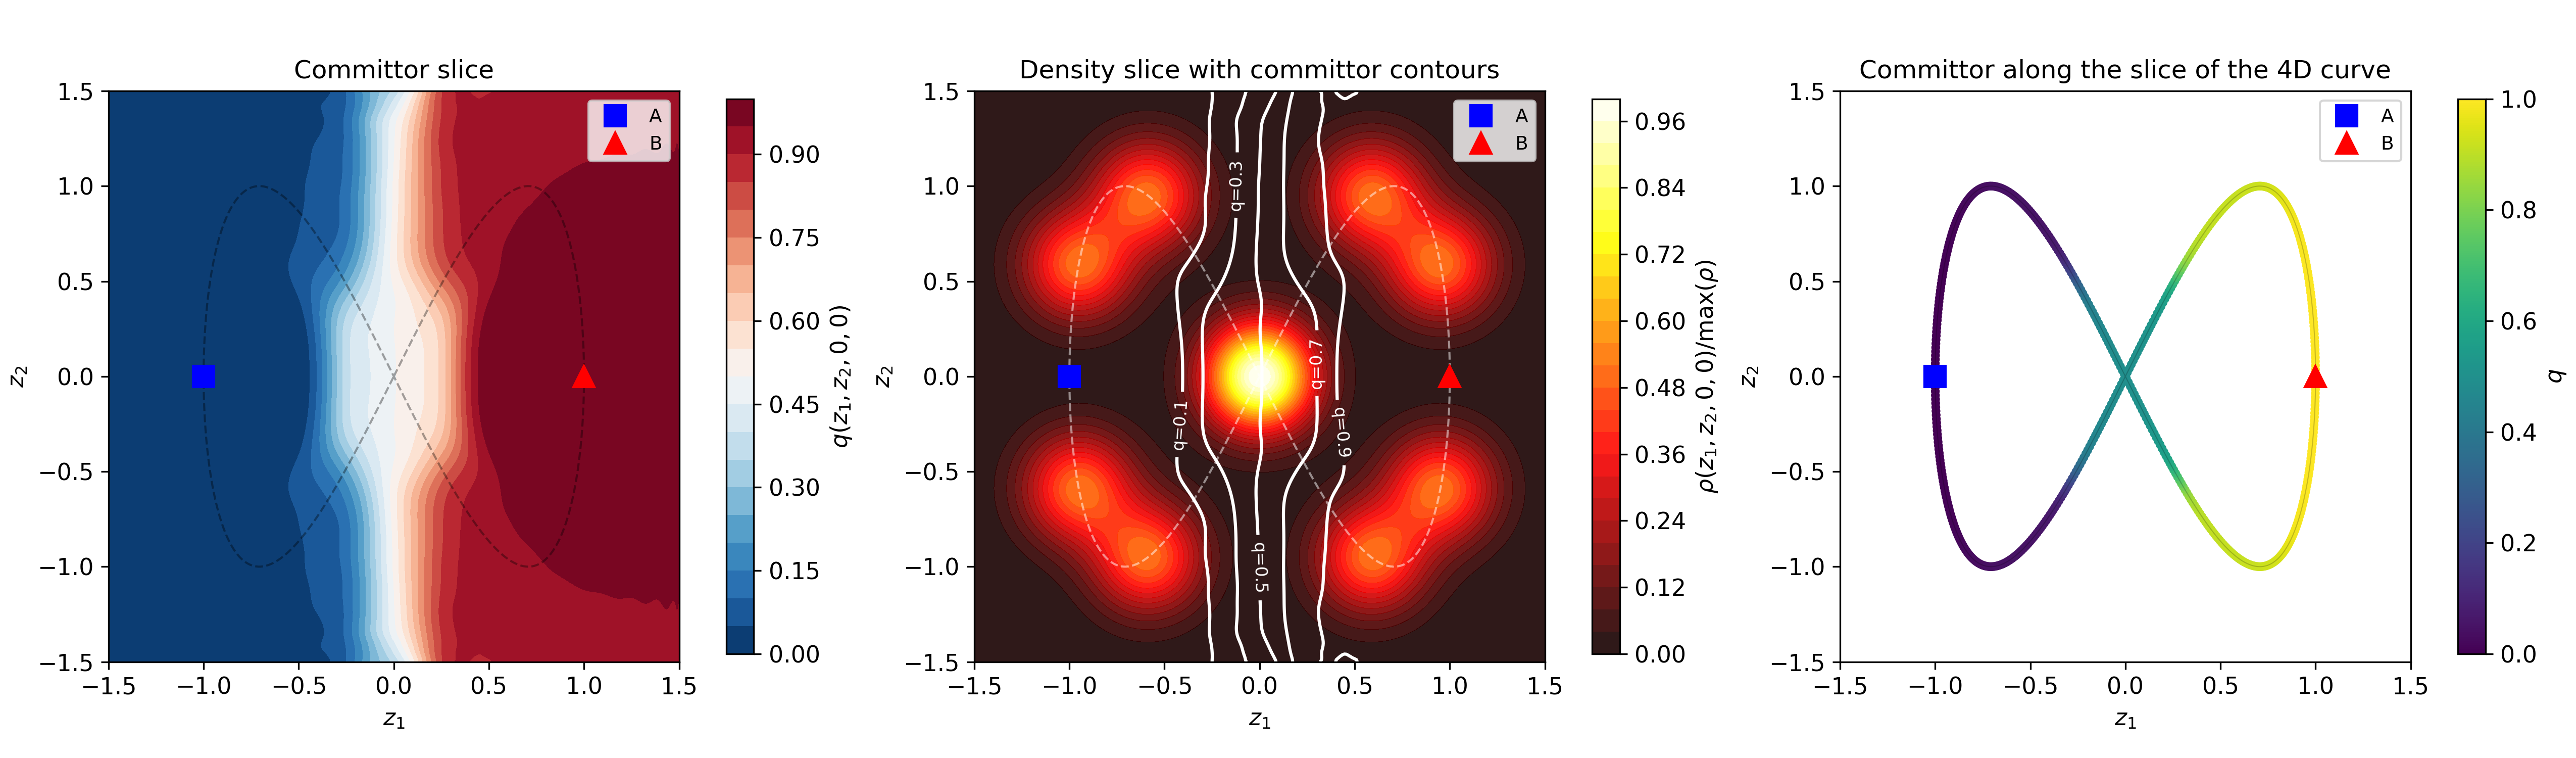
\includegraphics[scale=0.4]{recovar_4d.png}
    \caption{The 4 dimensional toy example with $N=10$. Qualitatively, these plots look pretty similar to the two dimensional case and so agree with what one would generally expect. We note that this result was highly sensitive to parameter selection so we hypothesize that better results can be obtained with more careful parameter tuning.}
\end{figure}

\section{Future}\label{sec:fut}
As discussed in \Cref{subsec:rec-con-dens}, RECOVAR must perform a density estimation in latent space to obtain the conformational density. Though we referred to this latent space as ``low-dimensional,'' concretely it tends to be somewhere around dimension 4-10. Even in dimension 4, however, parametric density estimation algorithms, such as kernel density estimation (KDE), begin to fail because of what is referred to as \emph{the curse of dimensionality}. This very general problem of using non-parametric methods to perform high-dimensional density estimation has been studied extensively. One method that we note for its connection to how we obtain the committor is \cite{ttde} (see, e.g. \url{https://github.com/matias-ma/tt-de} for an implementation of this). This algorithm essentially assumes that the underlying density has a TT expansion as in \cref{eq:tt-basis} and then minimizes the negative log-likelihood by running a gradient descent on the coefficient cores. Not only does using such an algorithm result in a more accurate estimation of the conformational density, but it also means that $p$ is \emph{a priori} in TT format (i.e. the conformational density is output in the form \cref{eq:tt-basis}). 

First and foremost, this means that we would no longer need to find the TT approximation of the estimated $p$, avoiding additional projection error and numerical instability. Second, it allows all quantities required for the committor computation to be expressed as tensor contractions, rather than numerical approximations of high-dimensional integrals.

From this perspective, TT density estimation and TT committor computation form a compatible pipeline since both rely on the same low-rank tensor structure and can share basis functions, tensor cores, and contraction routines. This suggests that an approach to cryo-EM heterogeneity, where both the density and the committor are learned in this TT format, may provide both computational and statistical advantages over other approaches.

This reformulation also hints at the convergence properties of this algorithm used to obtain the committor function. The ALS scheme used to solve \cref{eq:full-tt-cmmttr} is guaranteed to converge to a stationary point within the chosen class of TT cores, but this guarantee is only meaningful if the target functions admit accurate low-rank approximations. In particular, if both the equilibrium density $p$ and the committor $q$ are well-approximated in TT format, then the overall procedure is consistent up to the chosen ranks. Thus, the key question is not separability in a strict sense, but rather the existence of \emph{low-rank approximations} for the functions of interest.

While exact separability is a restrictive assumption, there is evidence that sufficiently regular functions admit efficient low-rank representations. In the bivariate case, results based on continuous LU decompositions (see, e.g., \cite{townsend}) show that analytic functions can be approximated with errors that decay rapidly with the rank. This suggests that regularity conditions such as analyticity of the effective free-energy landscape may, in practice, justify a TT approximation. A proof of this claim under suitable assumptions is omitted here and we defer a more detailed treatment to future work.

\section{A Toy Example: The Ginzburg-Landau Field}\label{sec:gl-example}

The two toy problems above are either exactly separable (the double well) or built by hand directly in tensor-train form (the mixture-of-Gaussians RECOVAR toy example): in both cases the equilibrium density is already known analytically, and already compatible with a low-rank format, before we ever try to solve for the committor. The pipeline we ultimately want for cryo-EM, however, must first \emph{estimate} the conformational density from samples, and only then solve for the committor on top of that estimate. As a closer, still fully-controlled proxy for that full pipeline, we consider a $d$-dimensional \emph{Ginzburg-Landau field}: a density that is genuinely non-separable and correlated across coordinates, has no closed-form TT representation handed to us in advance, and -- unlike a real cryo-EM latent density -- has a known ground truth we can validate the whole pipeline against. This model, and our parametrization of it, follows Peng, Khoo, and Wang \cite{vrs}, who use it as a standard hard benchmark for tensor-train density estimation.

\subsection{The model}
Physically, this is the standard lattice (real, scalar) Ginzburg-Landau free energy for an order-parameter field undergoing a symmetry-breaking phase transition. Concretely, we place $d$ scalar variables $x_1,\ldots,x_d$ on a chain, with fixed (zero) values $x_0=x_{d+1}=0$ at the two ends, and define the energy
\begin{align}
    U(\boldsymbol{x}) = \beta\left[\sum_{i=0}^{d}\frac{\lambda}{2}\left(\frac{x_{i+1}-x_i}{h}\right)^2 \;+\; \sum_{i=1}^d \frac{1}{4\lambda}(x_i^2-1)^2\right], \qquad h = \frac{1}{d+1},
\end{align}
with equilibrium density $p(\boldsymbol{x})\propto\exp(-U(\boldsymbol{x}))$, as usual for $\beta=1/T$. Each site's own term $(x_i^2-1)^2/(4\lambda)$ is a double well with minima at $x_i=\pm1$: left alone, every coordinate would independently prefer to sit in one of two ``phases.'' The first (gradient) term instead couples neighboring sites, penalizing the discretized derivative $(x_{i+1}-x_i)/h$; it is a discretization of $\int(\lambda/2)\,x'(s)^2\,ds$, and represents the energetic cost of an interface between a stretch of the chain sitting near $-1$ and a stretch sitting near $+1$. A small $\lambda$ makes this interface cheap to bend but expensive to leave the wells for, so the chain strongly prefers to be locally ordered -- close to one of the two spatially uniform ground states $\boldsymbol{x}\approx(-1,\ldots,-1)$ or $\boldsymbol{x}\approx(+1,\ldots,+1)$ -- with most of the remaining probability mass sitting in configurations containing a single domain wall somewhere along the chain rather than a fully disordered configuration. This is exactly what is visible in the estimated 2D marginals of \Cref{fig:gl-pipeline}: the two neighboring coordinates shown are each individually bimodal (bistable near $\pm1$) and correlated with each other, but not perfectly locked together, since a domain wall can sit between them.

This is, up to notation, the same free energy Ginzburg and Landau originally wrote down for the superconducting phase transition \cite{ginzburglandau}, generalized by Landau's mean-field theory of continuous, symmetry-breaking phase transitions to any scalar (or vector) order parameter; the same double-well-plus-gradient structure recurs throughout condensed matter physics, e.g.\ describing magnetic domains in a ferromagnet, phase coexistence and coarsening in an alloy (where the discretized, gradient-flow version of exactly this energy is the Allen-Cahn equation \cite{allencahn}), and structural or ferroelectric phase transitions in some semiconducting crystals, where the order parameter is a lattice distortion or polarization rather than a magnetization. So while the model is not \emph{specifically} a model of semiconductors -- Ginzburg-Landau theory's best-known application is superconductivity, and the discrete chain here is closer in spirit to a 1D ferromagnet or an Allen-Cahn interface model -- the same double-well-plus-gradient mathematics does genuinely recur in semiconductor physics wherever a structural or ferroelectric phase transition is involved.

\subsection{Why the committor is the interesting object here}
Because the density concentrates near the two uniform configurations $\boldsymbol{x}_A\approx(-1,\ldots,-1)$ and $\boldsymbol{x}_B\approx(+1,\ldots,+1)$, these are the natural pair of metastable states for a committor problem, exactly as in the double-well example, but now genuinely correlated rather than a product of $d$ independent copies of the same 1D problem. The committor $q(\boldsymbol{x})$ -- $\approx 0$ deep in the $A$ basin, $\approx 1$ deep in the $B$ basin -- then answers a nucleation-and-growth question: starting from a partially-ordered chain configuration $\boldsymbol{x}$ (e.g.\ one containing a domain wall part-way along its length), what is the probability that Langevin fluctuations complete the transition to the uniform $+1$ phase before they instead relax back to the uniform $-1$ phase? Level sets of $q$ therefore pick out the \emph{critical configurations} of this phase transition -- chain profiles that are, in a precise probabilistic sense, equally likely to finish flipping or fall back -- playing the same role here that a transition state plays in a chemical reaction, but for the growth of a domain wall rather than the rearrangement of a molecule. This is a useful diagnostic in its own right for phase-transition kinetics (nucleation, magnetization reversal, spinodal decomposition), and it is a natural stress test for our pipeline: unlike the earlier toy examples, both the density \emph{and} the committor here have real spatial structure induced by the chain's correlations, rather than being assembled from independent or hand-picked low-rank pieces.

\subsection{Sanity check: the committor scales to higher $d$}
Before estimating anything from data, we first check that our TT/Tucker committor solver itself behaves correctly on this genuinely correlated density, using the true, analytic Ginzburg-Landau potential throughout. \Cref{fig:gl-tt20,fig:gl-tucker5} show the training loss and the resulting committor along the straight-line path from $\boldsymbol{x}_A$ to $\boldsymbol{x}_B$, for a TT solve at $d=20$ (rank 6) and a Tucker solve at $d=5$ (rank 4) respectively -- per this project's convention of TT as the primary, linearly-scaling format and Tucker as a secondary showcase in the $3$--$7$D band. Both recover the expected qualitative signature of a committor -- $q\approx0$ at $\boldsymbol{x}_A$, a smooth sigmoidal rise, and $q\approx1$ at $\boldsymbol{x}_B$ -- and the 2D slices in the rightmost panels show the same domain-wall-driven structure as the density itself. The $d=20$ TT solve overshoots slightly past $1$ at $\boldsymbol{x}_B$ (\Cref{fig:gl-tt20}); as in the earlier toy examples, we found this kind of overshoot sensitive to the rank and $\rho$-continuation schedule, and did not tune further.

\begin{figure}[H]
    \centering
    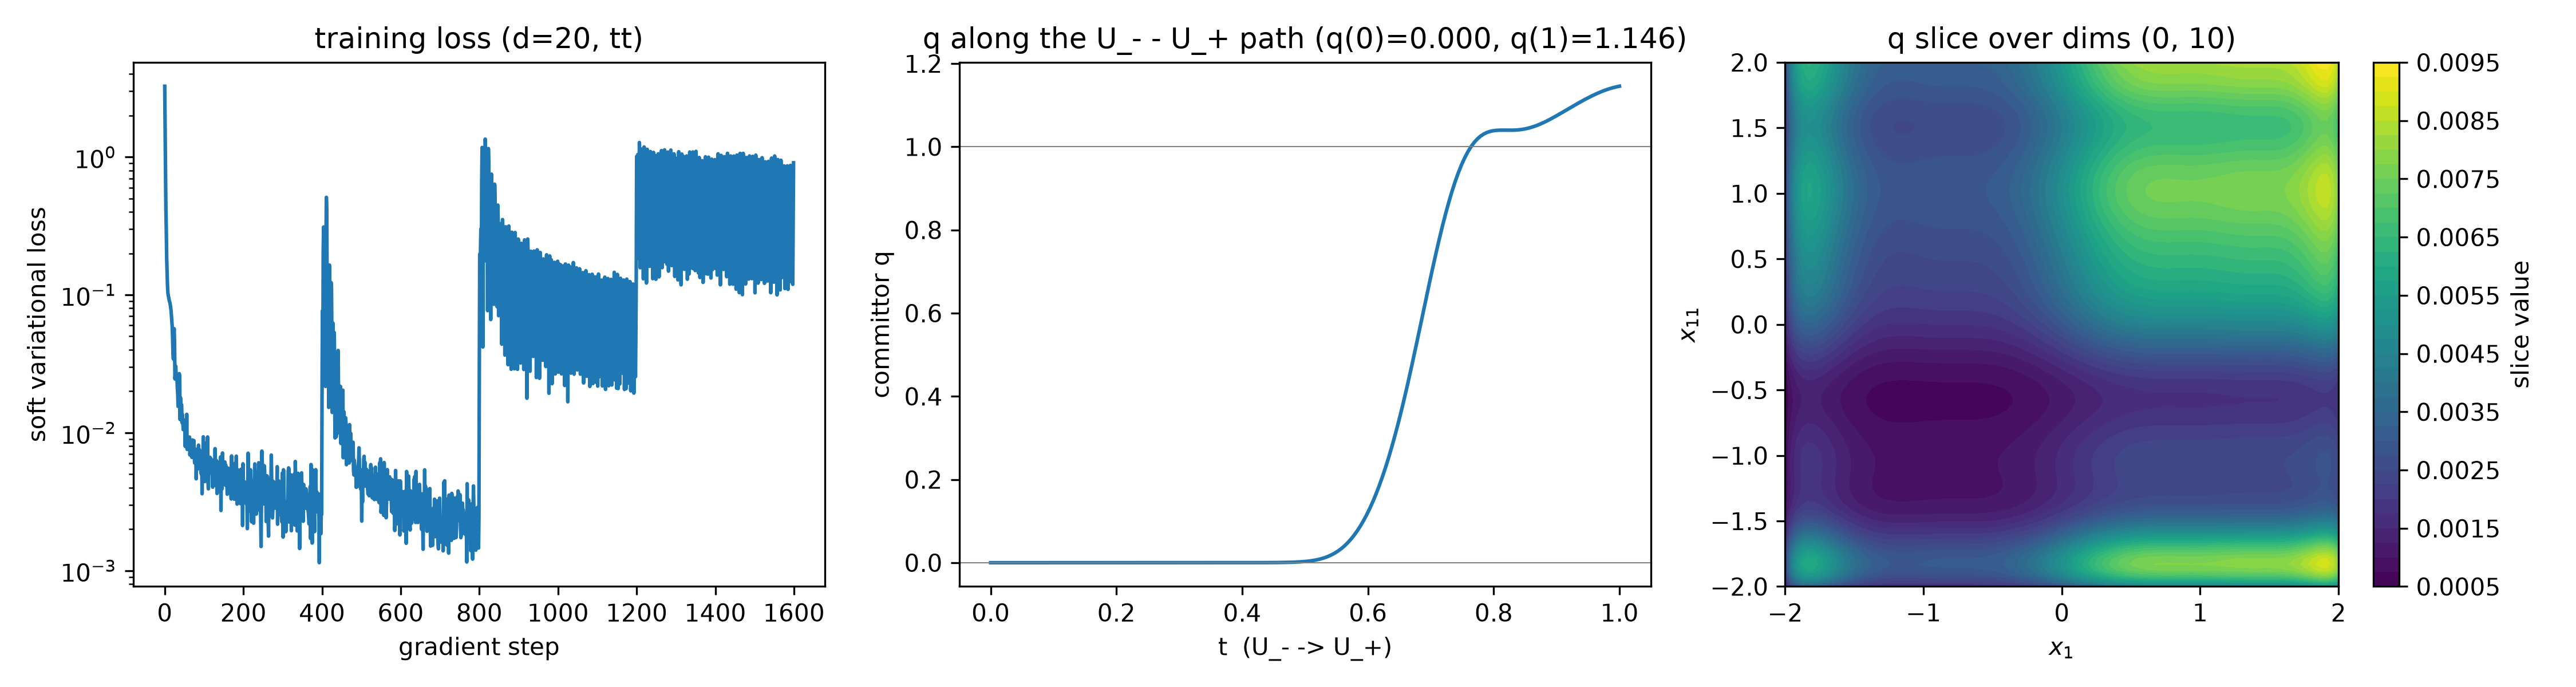
\includegraphics[width=0.95\linewidth]{ginzburg_landau_tt_d20.png}
    \caption{Committor solved in TT format directly from the true Ginzburg-Landau potential at $d=20$ (rank 6): training loss, the committor along the $\boldsymbol{x}_A\to\boldsymbol{x}_B$ path, and a 2D slice of $q$ over two of the chain's coordinates.}
    \label{fig:gl-tt20}
\end{figure}

\begin{figure}[H]
    \centering
    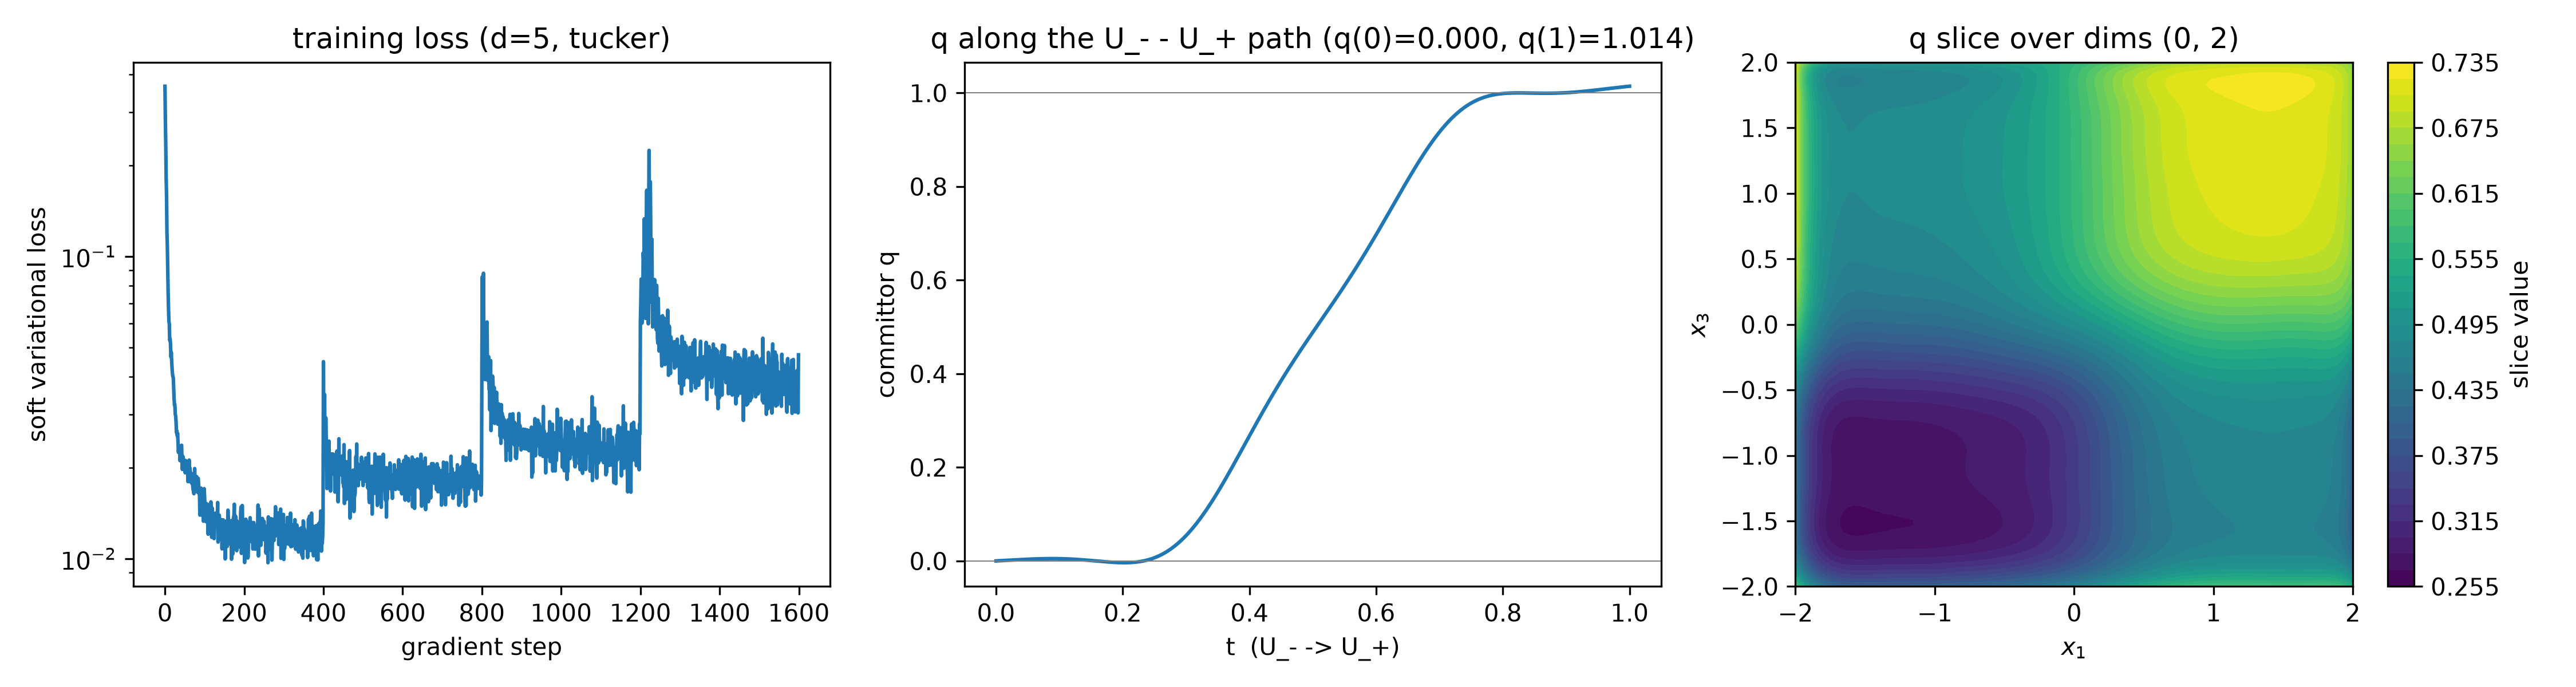
\includegraphics[width=0.95\linewidth]{ginzburg_landau_tucker_d5.png}
    \caption{The same experiment in Tucker format at $d=5$ (rank 4), in the $3$--$7$D band where a dense Tucker core is still cheap.}
    \label{fig:gl-tucker5}
\end{figure}

\subsection{The full pipeline: estimating the density, then the committor}
We now use this model to dry-run the full pipeline this project is aimed at: estimate a density from samples alone (rather than assuming it is already known or already in TT form), locate its metastable basins directly from that estimate, and only then solve for the committor between them -- comparing throughout against a committor solved from the true, analytic potential. Concretely, at $d=10$ with $n=100{,}000$ observed samples: we draw samples from $p$ by Metropolis-Hastings, fit a squared-Chebyshev-TT density to them with our \texttt{ft-de} density-estimation code, and repeat this after corrupting the samples with a substantial \emph{colored} observation noise model -- each observation's noise drawn from its own randomly sampled, heteroscedastic and pairwise-correlated covariance (100 such covariances sampled overall, giving per-coordinate noise standard deviations ranging from $0.22$ to $1.18$ against the density's own $\pm1$ scale, and pairwise correlations $\rho$ ranging from $0.35$ to $0.84$), then fit the noisy data both naively (an untrained Gaussian-KDE cross-approximation, since at this noise level training a no-deconvolution model barely improves on that untrained init) and using \texttt{ft-de}'s noise-deconvolution procedure against the corresponding averaged noise kernel. For the clean and deconvolved-noisy fits, we then locate the two basins directly from the fitted density -- with no reference to the true potential -- by averaging the most extreme $2\%$ of training points along the chain's mean order parameter (denoising a single noisy observation's idiosyncrasies the same way any other statistic benefits from averaging) and refining that estimate by a short local optimization, then solve the committor from each estimated density with the same TT machinery as above, again alongside a committor solved from the true potential as ground truth. \Cref{fig:gl-pipeline} shows the whole pipeline end to end, panels (a)--(f): the true density (an \emph{exact} 2D marginal, via the same transfer-operator recursion used for the normalizing constant -- not a sample histogram, which would itself carry its own sampling noise), the noise kernel, the resulting noisy observations (a histogram, since these really are individual noisy samples), the deconvolved density fit, and the committor solved on top of it (panel (e), using the same sequential viridis color scale as the density panels rather than a diverging one, so density and committor read as one consistent visual language), each annotated with its own fit statistics; a second row repeats (a)--(d) as their matching 1D marginals and adds the basin-to-basin committor path for all three potentials overlaid; panel (f) is a density-estimation-quality bar chart across all fits.

Deconvolution here is a genuinely ill-posed inverse problem, and getting a good fit took real care. Our first attempt reused \texttt{ft-de}'s own Tikhonov-regularized recipe (penalizing the fitted density's noise-convolved amplitude, calibrated to a per-axis target budget) at the same rank/degree as the rest of the pipeline ($10$/$19$): its relative $L^2$ error against the true density turned out to be \emph{non-monotonic} in training length regardless of the regularization strength tried, improving for roughly the first $1{,}000$--$2{,}000$ steps and then degrading sharply and irrecoverably as training continued to overfit the noise -- and this degradation was invisible to the validation negative log-likelihood used for checkpoint selection, which kept improving for thousands of steps past the point where the reconstructed density had already begun diverging. Stronger regularization budgets delayed and softened, but never eliminated, this failure: the best minimum error reachable this way (relative $L^2\approx0.35$) was comparable to what the fix below ultimately achieves, but only inside a narrow, hand-tuned early-stopping window a few hundred steps wide -- training even modestly past it made the fit rapidly, substantially worse. We instead adopted \texttt{ft-de}'s own separately-validated recipe for a comparably heterogeneous, correlated noisy-Ginzburg-Landau benchmark (its \texttt{gl\_covariance\_mixture} experiment): a Sobolev-$H^1$ amplitude-smoothness penalty on the fitted density itself, together with a markedly \emph{smaller} tensor-train rank ($4$, vs.\ $10$ elsewhere in this pipeline) and \emph{higher} Chebyshev degree ($24$, vs.\ $19$) for the deconvolution stage specifically. Re-tuning only the smoothness weight for our own (more heterogeneous) noise model, this recipe behaves qualitatively differently from the Tikhonov one: relative $L^2$ error drops for about $1{,}000$ steps and then sits on a broad, \emph{stable} plateau ($0.33$--$0.39$) for the remaining $7{,}000$ steps tried, rather than blowing up -- so plain validation-NLL checkpoint selection is safe here, with no hand-tuned stopping point needed. The resulting deconvolved fit reaches a relative $L^2$ error of $0.356$, roughly $2.8\times$ better than the untrained naive baseline's $0.998$ (and, for reference, short of the clean, noise-free fit's $0.014$) -- see the bar chart in \Cref{fig:gl-pipeline}.

Despite that nontrivial residual error in the deconvolved density, the committor solved on top of it still recovers the same qualitative sigmoidal shape as the true-potential and clean-density committors, visible in the basin-to-basin path plot in \Cref{fig:gl-pipeline}: soft-variational final training losses of $0.059$ (true potential), $0.066$ (clean-estimated density), and $0.083$ (deconvolved-noisy-estimated density) -- only about $40\%$ higher than the true-potential committor, and close to the clean-density committor's own loss, despite the much larger gap in the underlying density's own accuracy. This suggests the committor is, at least in this example, a comparatively forgiving quantity to compute on top of an imperfect density estimate -- exactly the property we would want for the eventual RECOVAR pipeline, where the input density will only ever be an estimate.

\begin{figure}[H]
    \centering
    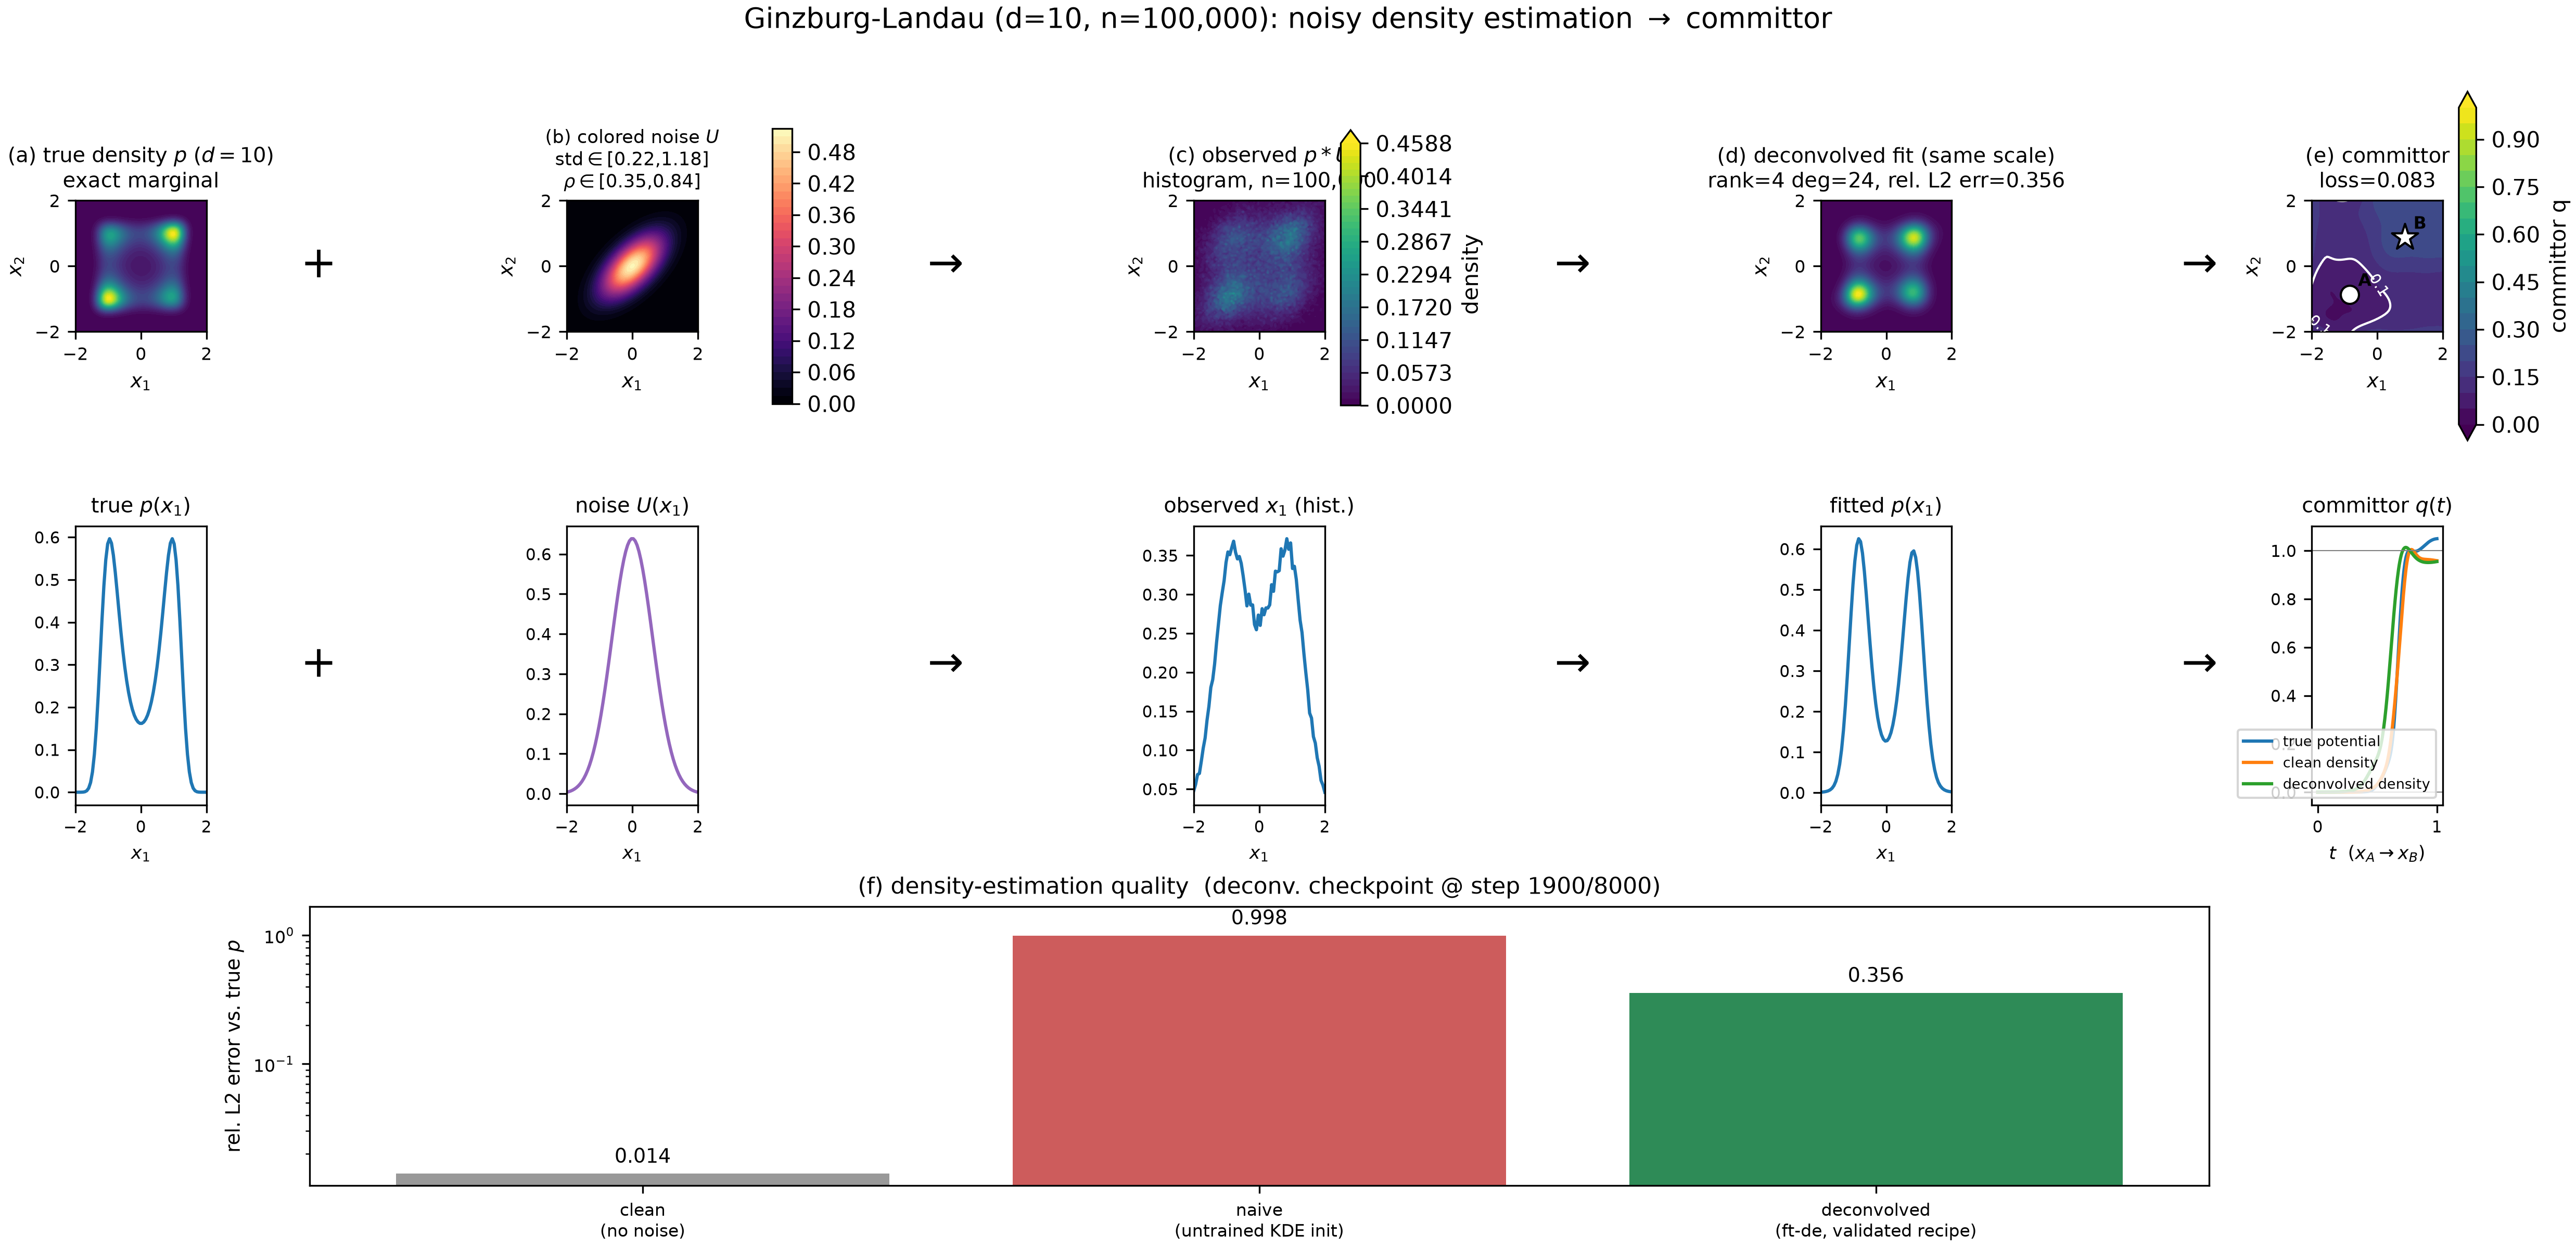
\includegraphics[width=0.95\linewidth]{ginzburg_landau_noisy_pipeline.png}
    \caption{The full pipeline on Ginzburg-Landau ($d=10$, $n=100{,}000$), end to end. Top row: (a) the true density's exact 2D marginal (transfer-operator recursion, not a histogram); (b) the colored (heteroscedastic, pairwise-correlated) noise kernel; (c) the resulting observed noisy data (histogram); (d) \texttt{ft-de}'s noise-deconvolved density fit (rank $4$, degree $24$, Sobolev-$H^1$ smoothness regularization), relative $L^2$ error $0.356$ (vs.\ $0.998$ untrained naive, $0.014$ clean, same color scale as (a)/(c)); (e) the committor solved on top of that fit -- with no reference to the true potential for either the basins or the density -- final loss $0.083$ (vs.\ $0.059$ true-potential and $0.066$ clean-density), using the same viridis color scale as the density panels. Middle row: the matching 1D marginals for (a)/(b)/(c)/(d), and the basin-to-basin committor path for all three potentials overlaid. Bottom: (f) density-estimation quality across all fits.}
    \label{fig:gl-pipeline}
\end{figure}

\subsection{The same pipeline without noise, as an ablation}
As a complementary, noise-free ablation at the same $d=10$, we also run the pipeline with no observation noise at all, using \texttt{ft-de}'s own dimension-tiered recipe (rank $10$, Chebyshev degree $19$, $4000$ NLL steps, $20000$ training points) unchanged -- a higher tensor-train rank than the noise-robustness-driven rank $4$ used for the noisy pipeline's deconvolution stage above, since without noise to regularize against there is no reason to shrink it. This isolates how much of the noisy pipeline's residual error is attributable to the noise/deconvolution step specifically, versus a capacity limit of the density-estimation machinery itself at this dimension. $d=10$, not \texttt{ft-de}'s own nominal ``high-dimension'' $d=20$ tier, is used deliberately here too: running \texttt{ft-de}'s own unmodified benchmark script ourselves at $d=8,10,14,20$ gives relative $L^2$ errors of $0.083$, $0.280$, $0.558$, and $1.018$ respectively -- i.e.\ its $d=20$ tier, as shipped, is actually \emph{worse} than its own Gaussian-KDE baseline ($1.018$ vs.\ $0.9997$) and evidently was never validated end to end; $d=10$ is the highest dimension we confirmed \texttt{ft-de}'s own settings actually work well at.

\Cref{fig:gl-clean-pipeline} shows this $d=10$ run: the TT density fit reaches relative $L^2$ error $0.280$ against the true density, a $3.5\times$ improvement over the Gaussian-KDE baseline's $0.972$ (KDE degrading toward uninformative as $d$ grows is exactly the curse-of-dimensionality behavior a low-rank tensor-train format is meant to avoid). The two metastable basins, again located directly from the fitted density with no reference to the true potential, land within a few hundredths of the true homogeneous states $\boldsymbol{x}_A\approx(-1,\ldots,-1)$, $\boldsymbol{x}_B\approx(+1,\ldots,+1)$ in every one of the 10 coordinates. The resulting committor's basin-to-basin path closely tracks the true-potential committor's (final soft-variational losses $0.084$ vs.\ $0.059$), again showing the committor solve itself tolerating the residual density-estimation error gracefully.

\begin{figure}[H]
    \centering
    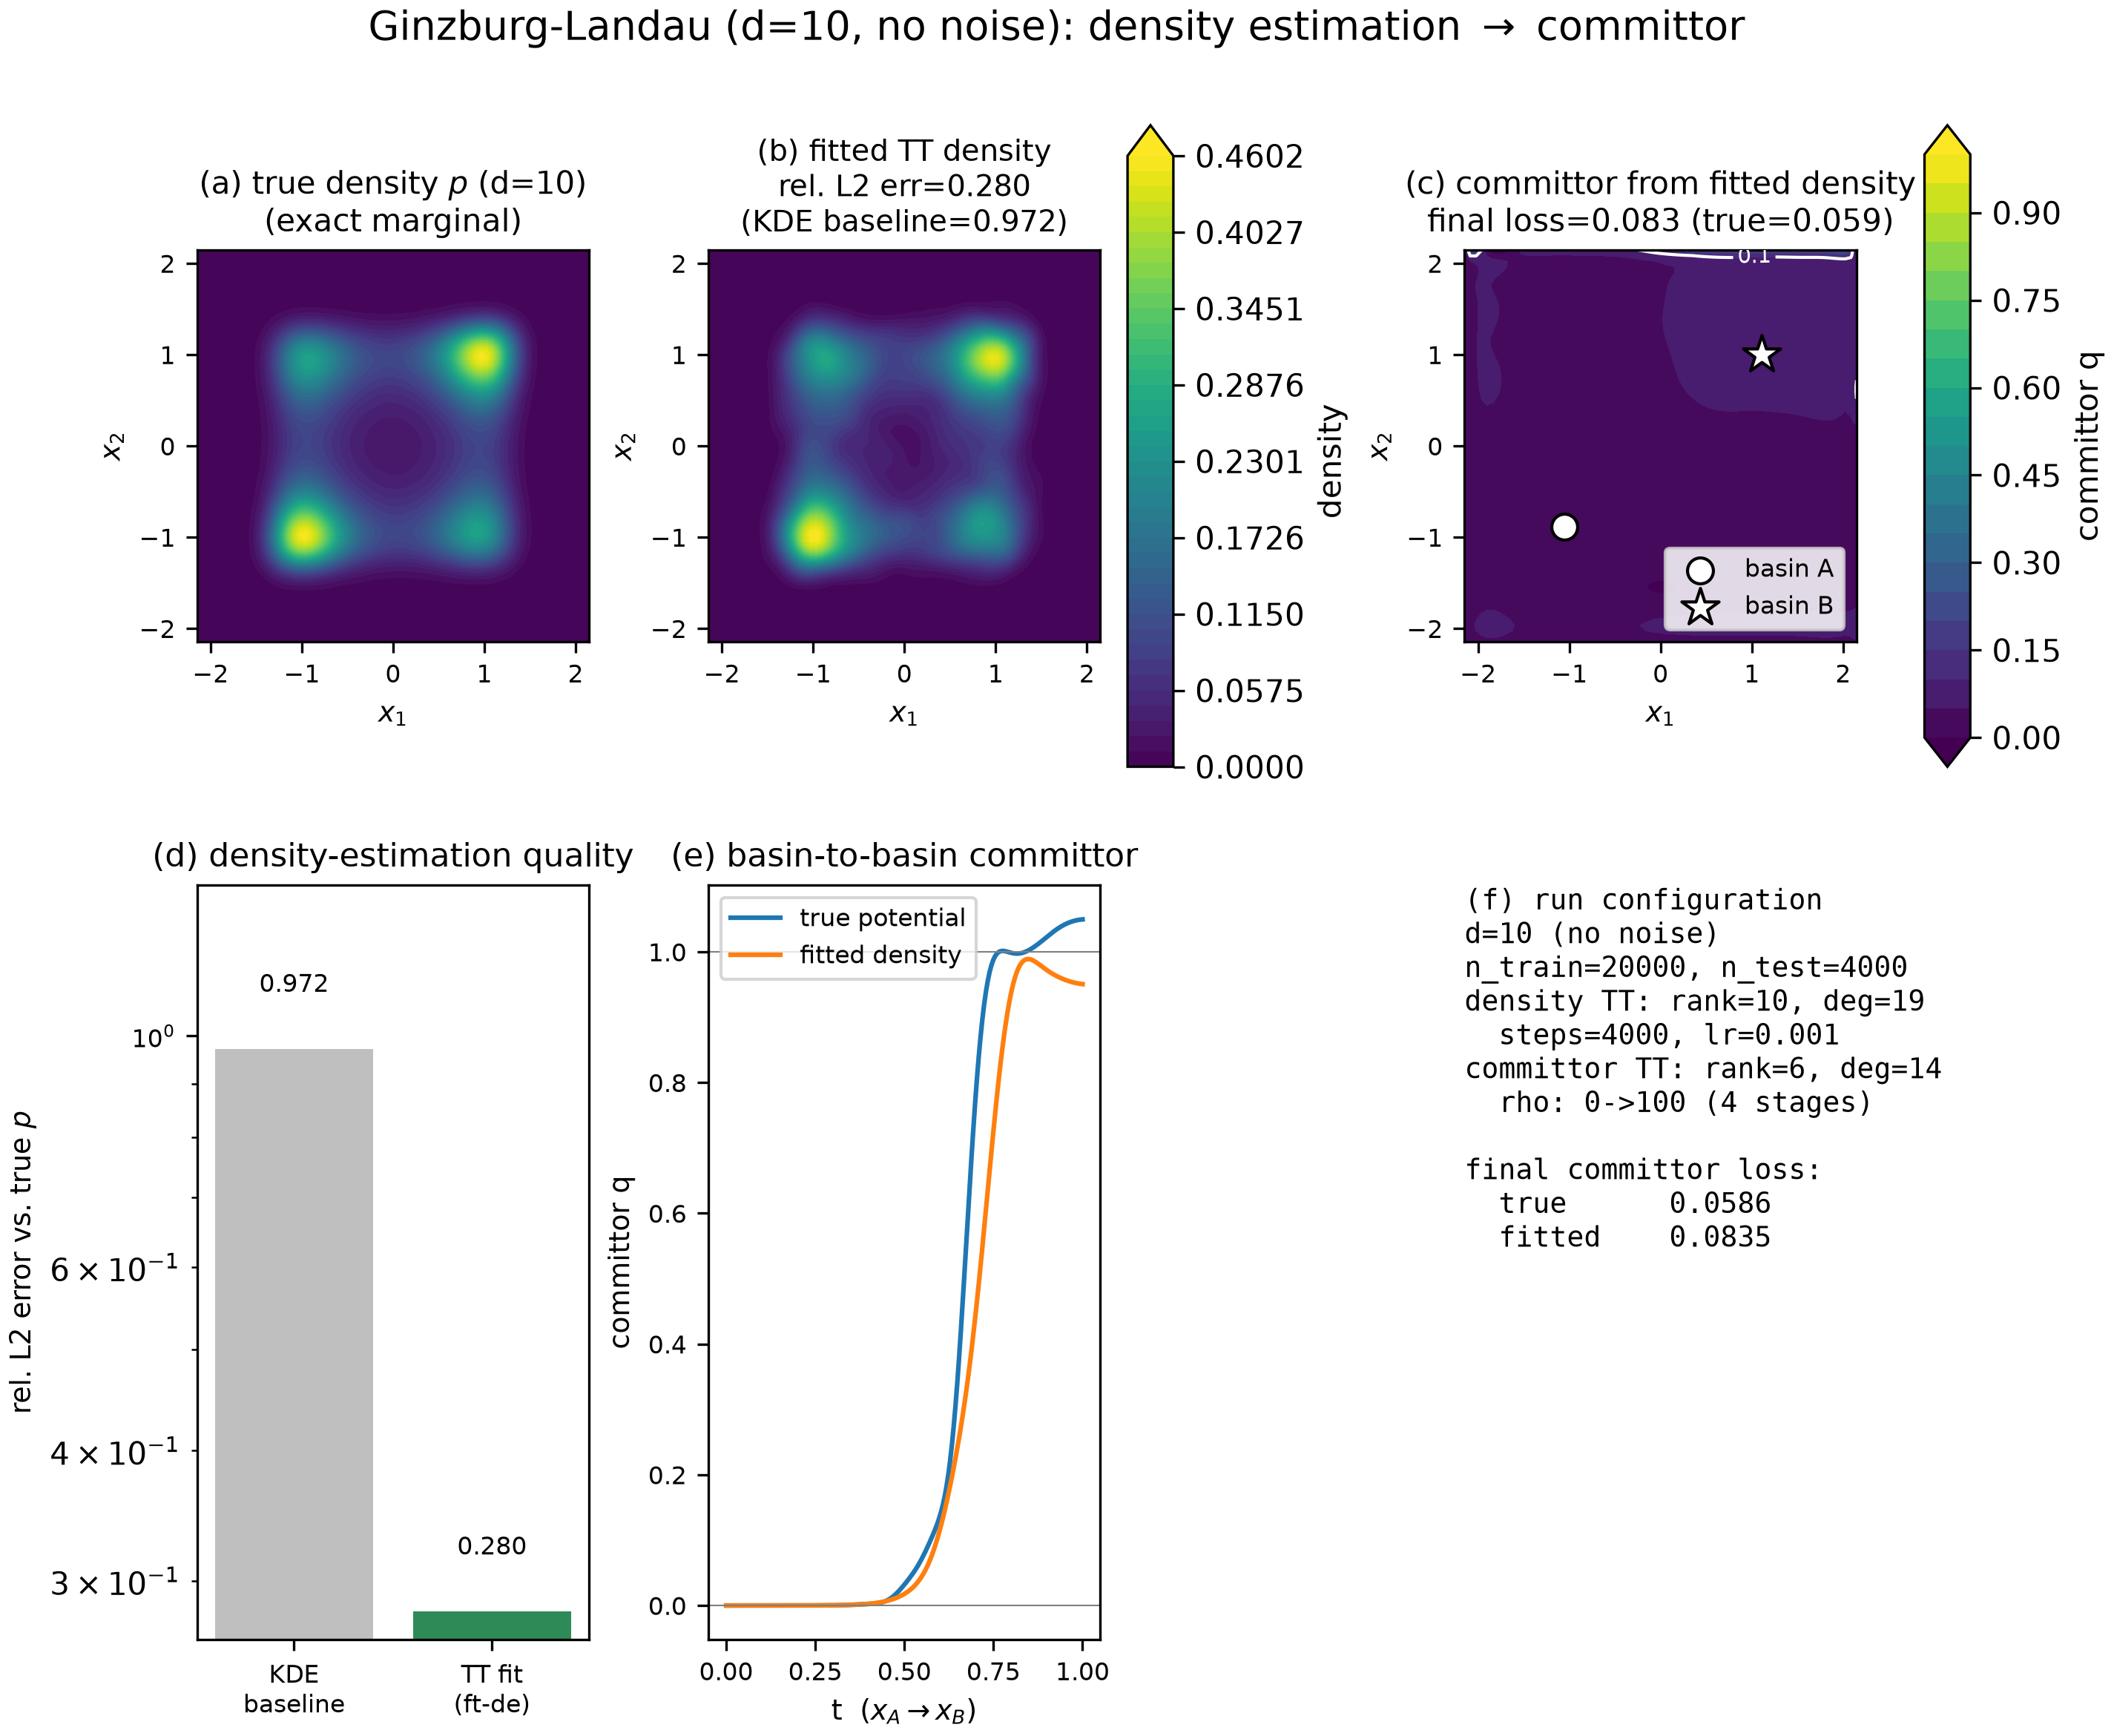
\includegraphics[width=0.95\linewidth]{ginzburg_landau_clean_pipeline.png}
    \caption{The same pipeline as \Cref{fig:gl-pipeline}, at the same $d=10$ but with no observation noise, using \texttt{ft-de}'s own validated dimension-tiered recipe unchanged (rank $10$, degree $19$ -- higher-capacity than the noise-robustness-driven rank $4$/degree $24$ used for \Cref{fig:gl-pipeline}'s deconvolution). (a) true density, exact marginal; (b) fitted TT density, relative $L^2$ error $0.280$ (vs.\ $0.972$ Gaussian-KDE baseline); (c) committor from the fitted density (viridis, same scale as (a)/(b)), final loss $0.083$ (vs.\ $0.059$ true-potential); (d) density-estimation quality (KDE baseline vs.\ TT fit); (e) basin-to-basin committor path, true potential vs.\ fitted density; (f) run configuration.}
    \label{fig:gl-clean-pipeline}
\end{figure}

I would like to thank Marc Aurèle Gilles for giving me the idea for this application.

\bibliographystyle{plain}
\bibliography{citations}

\end{document}
